\documentclass[11pt, english]{beamer}
\usepackage{babel}
\usepackage[T1]{fontenc}
\usepackage[utf8]{inputenc}

%Justificación del texto
\usepackage{ragged2e}
\justifying

\usepackage{pgf,pgfpages}
\usepackage{pgffor} % For loops
\usepackage{tikz}
\usetikzlibrary{arrows,shapes,backgrounds,calc}

\usepackage{graphicx}
\usepackage{colortbl}
\usepackage{units}

% Fuente caligráfica en entornos matemáticos
\usepackage[cal=boondox,scaled=1.15]{mathalfa}

%% Beamer style >>>>>>>>>>>>>>>>>>>>>>>>>
\mode<presentation>
{
  \usetheme{PHD}
  \setbeamercovered{transparent}
  \setbeamertemplate{items}[square]
}

%\usefonttheme[onlymath]{serif}

\beamertemplatenavigationsymbolsempty

\defbeamertemplate{enumerate item}{mycircle}
{
  %\usebeamerfont*{item projected}%
  \usebeamercolor[bg]{item projected}%
  \begin{pgfpicture}{0ex}{0ex}{1.5ex}{0ex}
    \pgfcircle[fill]{\pgfpoint{-0.1pt}{.65ex}}{1.1ex}
    \pgfbox[center,base]{\color{PHDyellowd}{\insertenumlabel}}
  \end{pgfpicture}%
}
[action]
{\setbeamerfont{item projected}{size=\scriptsize}}
\setbeamertemplate{enumerate item}[mycircle]

\title{Aplicaciones de la IA al Mundo Real}
\author{Álex Pérez Fernández, Rafa Rodríguez Galván}


% PDFLaTeX font choosing
\usepackage[default, scale=1.0]{lato}

% \usepackage{array, multirow, rotating} % booktabs: toprule, midrule...
\usepackage{array,booktabs,tabularx}

\usepackage{current-definitions}
\usepackage{neural-networks}

\newtheorem{remark}{Remark}
\newtheorem{proposition}{Proposition}
%\newtheorem{theorem}{Theorem}

% Presentation goodies >>>>>>>>>>>>>>>>>>>>>>>>>>>>
\newcommand<>{\myframed}[1]{\alt#2{\tikz[phd] \node[box] {#1};}{{#1}}}
\newcommand<>{\myframedAlert}[1]{\alt#2{\tikz[phdB] \node[boxB] {\color{black}#1};}{{#1}}}
\newcommand<>{\framedmath}[1]{%
\alt#2{\tikz[phd] \node[box] {\ensuremath{#1}};}{\ensuremath{#1}}}
\newcommand{\framedB}[1]{\tikz[phd] \node[boxB] {#1};}
\newcommand{\framedmathB}[1]{\framedB{\ensuremath{\displaystyle{#1}}}}
\newcommand{\ver}[1]{\footnote{See #1}}
\newcommand{\cita}[1]{{\color{PHDgray}\cite{#1}}}
\newcommand\cellalert[2]{\only<#1>{\cellcolor{PHDyellow}}\alt<#1>{\textbf{#2}}{#2}}
\newcommand{\soften}[1]{{\color{PHDgray}#1}}
\newcommand{\rowalert}[7]{%
    \cellalert{#1}{#2} & \cellalert{#1}{#3} &
    \cellalert{#1}{#4} & \cellalert{#1}{#5} &
    \cellalert{#1}{#6} & \cellalert{#1}{#7}}

% \usepackage{wasysym}
% \newcommand{\good}{{\color{PHDgreen}$\CIRCLE$}} %\blacksmiley
% \newcommand{\bad}{{\color{PHDred}$\CIRCLE$}}
\usepackage{pifont, fontawesome}
\newcommand{\good}{{\color{PHDgreen}\ding{52}}}
\newcommand{\bad}{{\color{PHDred}\ding{56}}}
\newcommand{\exclamation}{{\large\color{PHDred}{\textbf{\itshape !}}}}
\newcommand{\question}{{\large\color{PHDred}{\textbf{\itshape ?}}}}
\newcommand\colorUnderLine[2][PHDyellow]{\color{#1}\underline{{\color{black}#2}}\color{black}\xspace}
\newcommand\gris[1]{{\color{PHDgray}#1}}
\newcommand\amarillo[1]{{\color{PHDyellow}#1}}
\newcommand\tiragris[1]{{\par\hfill\small\gris{#1}}}
\newcommand\point{\alert{\faHandORight}\xspace}
%<<<<<<<<<<<<<<<

\setcounter{tocdepth}{1}


%
% Bibliography
%
%\usepackage{natbib}

% To list each bibliographic entry in a line
\setbeamertemplate{bibliography entry title}{}
\setbeamertemplate{bibliography entry location}{}
\setbeamertemplate{bibliography entry note}{}

% ... end of preamble.

\AtBeginSection{\frame{\sectionpage}}

\colorlet{inputcolor}{green!60!black}
\colorlet{hiddencolor}{blue!60!black}
\colorlet{outcolor}{red!60!black}

%--------------------------------------------------------------
\begin{document}
%--------------------------------------------------------------

% Tikz style and beamer template ------->>>
\tikzstyle{every picture}+=[remember picture]
\tikzstyle{na} = [baseline=-.5ex]
\tikzstyle{phd} = [baseline=-.6ex,
  box/.style={rectangle, draw=PHDblueC, thick, fill=PHDblueA,
    align=center, rounded corners, minimum height=1.6em},
  boxB/.style={rectangle, draw=PHDredA, thick, fill=PHDblueA,
    align=center, rounded corners, minimum height=1.6em}]
\tikzstyle{phdB} = [baseline=-.7ex,
  box/.style={rectangle, draw=PHDblueC, thick, fill=PHDblueA,
    align=center, rounded corners, minimum height=1.6em},
  boxB/.style={rectangle, draw=PHDredA, thick, fill=PHDblueA,
    align=center, rounded corners, minimum height=1.6em}]
\tikzstyle{myarrow} = [->,>=latex, PHDredA, shorten >=4pt,
  opacity=.6, line width=0.6mm]
\tikzstyle{myarrow2} = [->,>=latex, PHDblueC, shorten >=4pt, opacity=.2, line width=0.4mm]
\tikzstyle{myarrow3} = [
     opacity=.7,
%    >=triangle 60,              % Nice arrows; your taste may be different
    node distance=6mm and 60mm, % Global setup of box spacing
    every join/.style={norm},   % Default linetype for connecting
                                % boxes
    line width=0.6mm,
    PHDredA,
    ->
    ]
\setbeamertemplate{background}
 {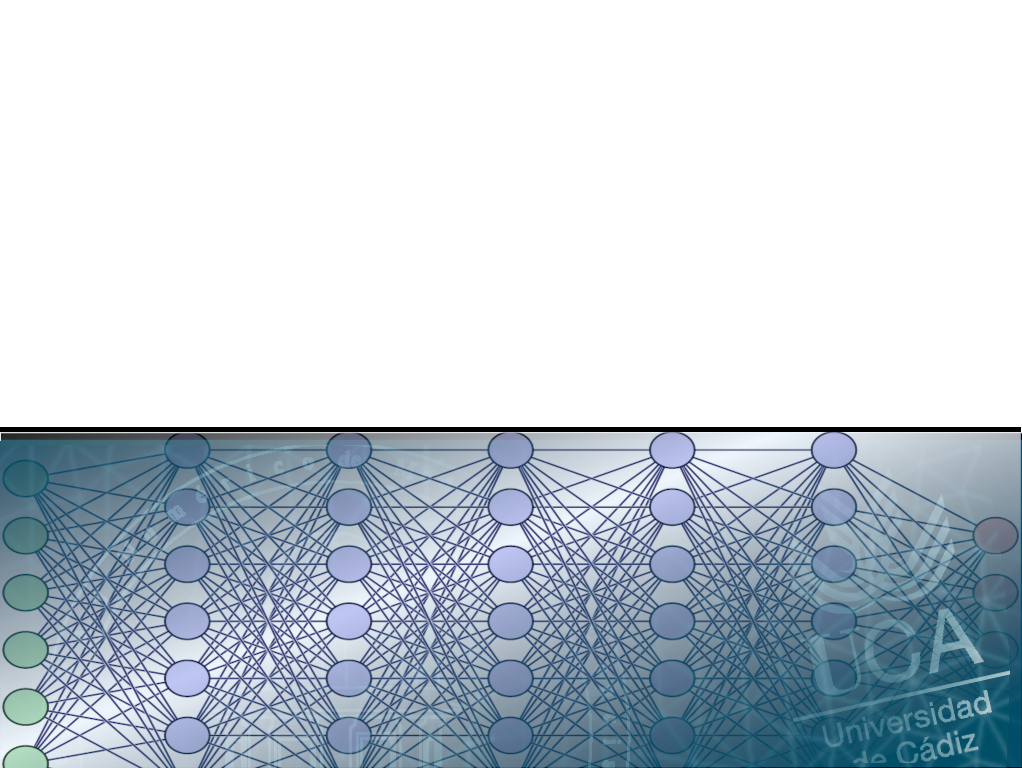
\includegraphics[width=\paperwidth,height=\paperheight]{frontpage_bg}}
\setbeamertemplate{footline}[default]
% <<<-------


% Write custom titlepage ------->>>
\begin{frame}
  \titlepage
  \vspace{5cm}
\end{frame}

% Set the background for the rest of the slides.
\setbeamertemplate{background}{}
 % {
\includegraphics[width=\paperwidth,height=\paperheight]{slide_bg}}


% Write all of the slides..........

% \begin{frame}{Outline}
%   \tableofcontents
% \end{frame}

% Start inserting infoline at the end
\setbeamertemplate{footline}[PHDtheme]
% <<<-------

\newcommand{\imgdir}{Undefined, use renewcommand!}

%--------------------------------------------------------------
\section{Redes Neuronales}
%--------------------------------------------------------------

\begin{frame}{Las Redes Neuronales...}
%--------------------------------------------------------------
  \vspace{-0.9em}
  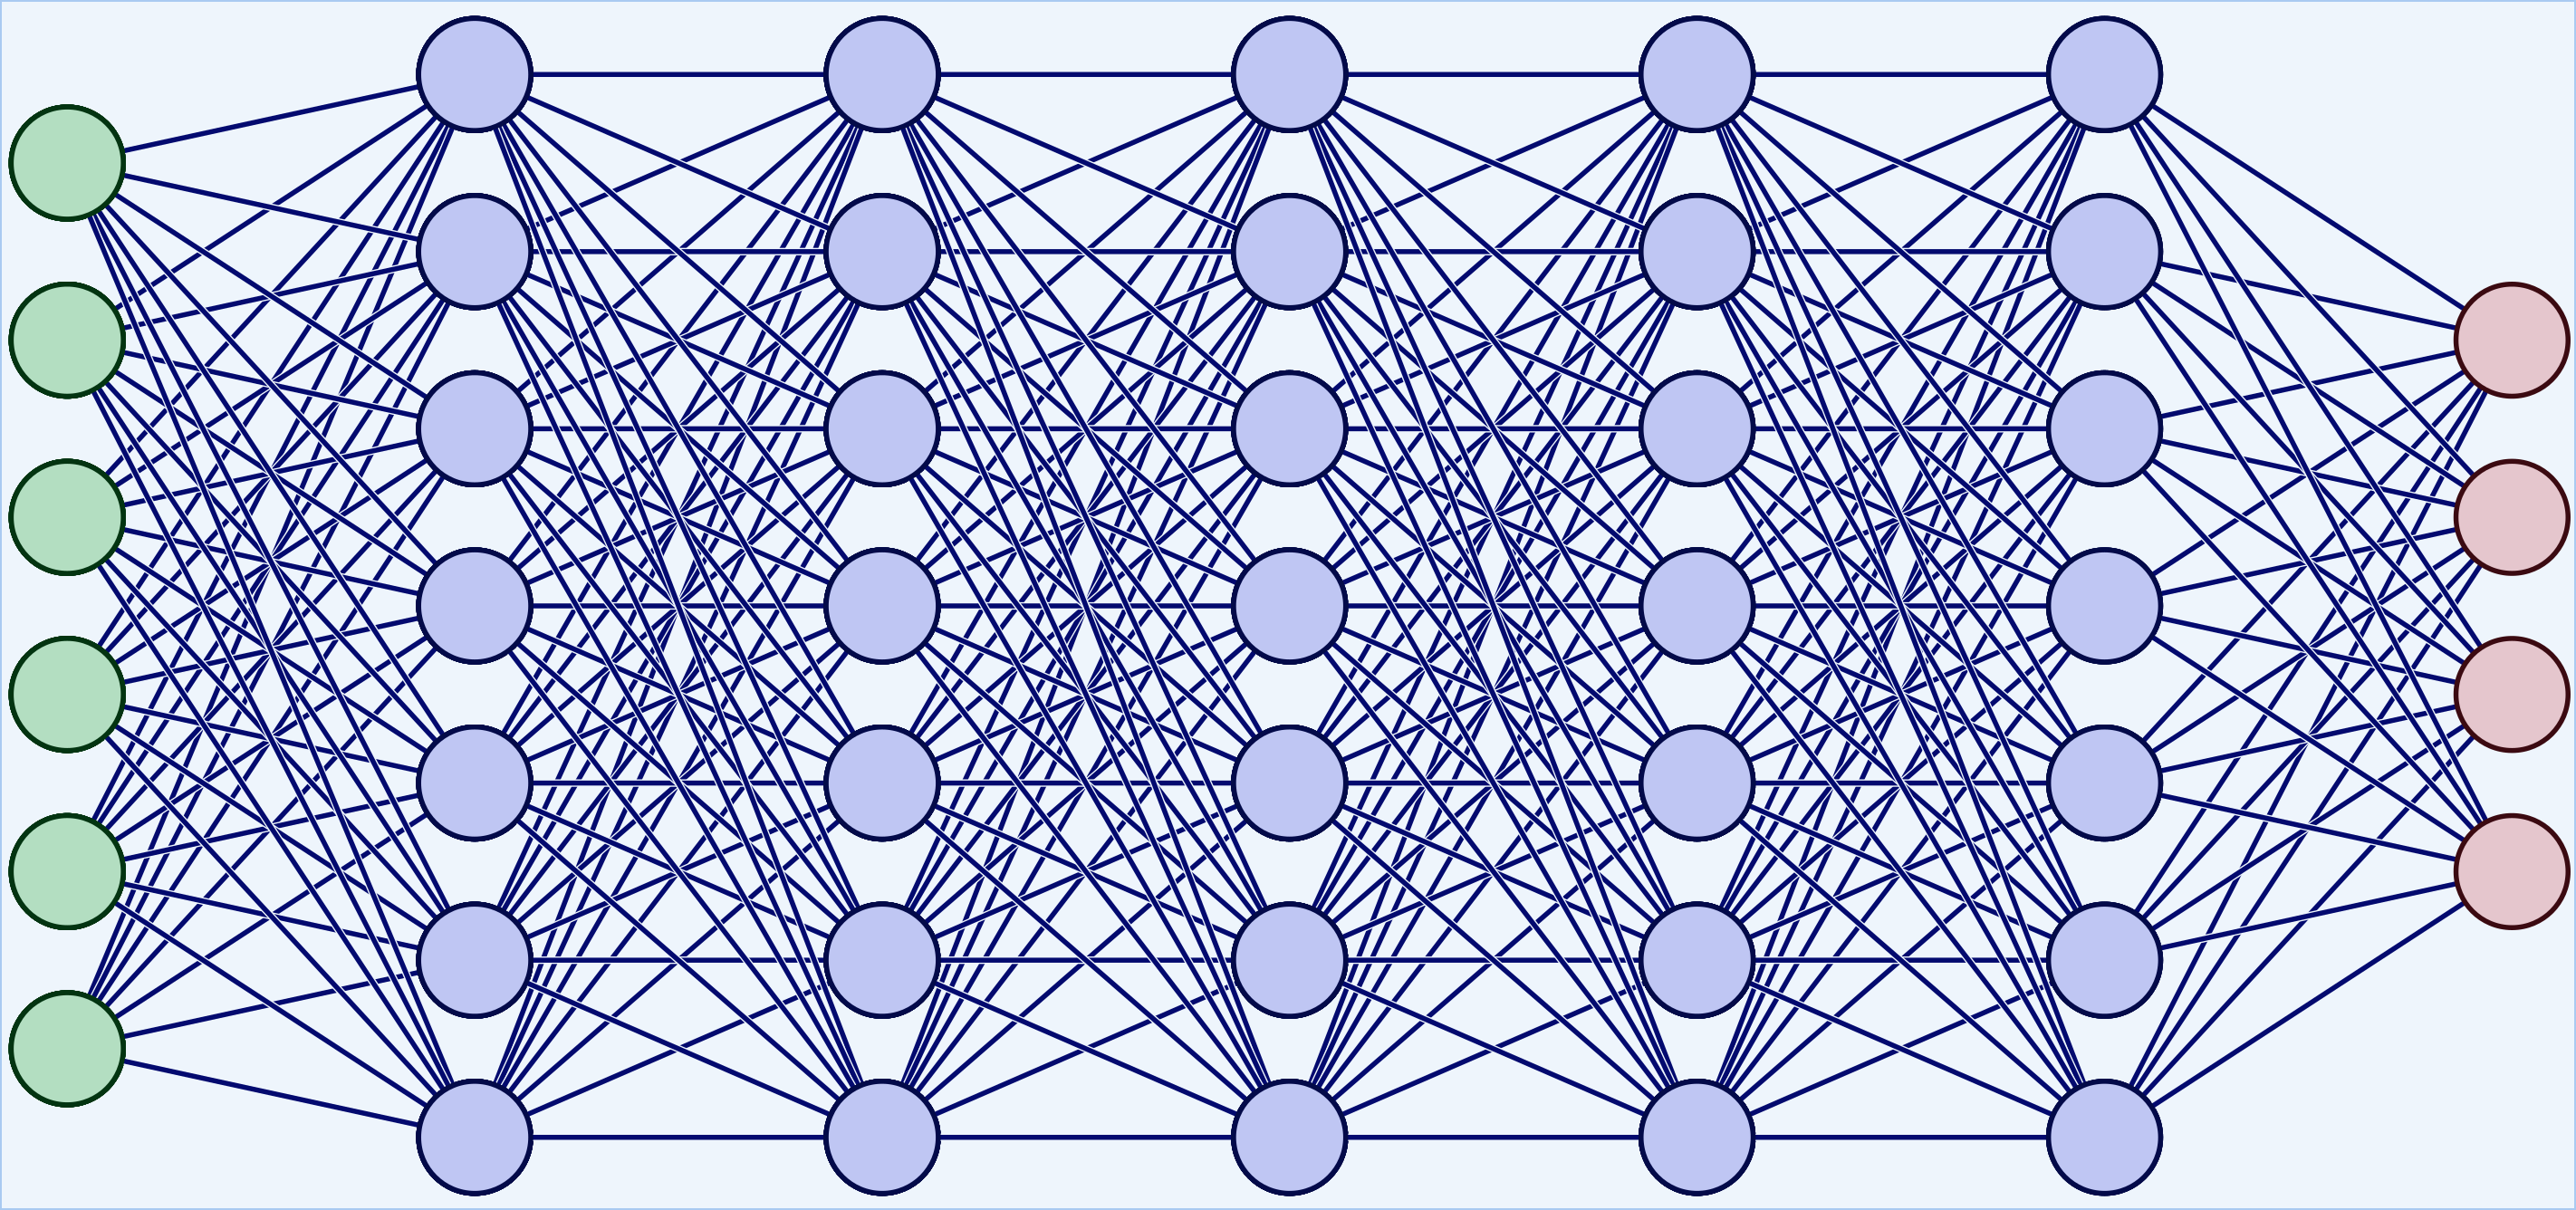
\includegraphics[width=0.95\linewidth]{deep-NN}
  \pause
  ~
  \vfill
  {\large\textbf{son artefactos matemáticos:}}
  \begin{gather*}
    {\color{inputcolor} \xx} \mapsto 
    {\color{hiddencolor}\ff_1({\color{inputcolor} \xx})} \mapsto 
    {\color{hiddencolor}\ff_2\circ \ff_1({\color{inputcolor} \xx})} \mapsto 
    % {\color{hiddencolor}\ff_3\circ \ff_2\circ \ff_1({\color{inputcolor} x})} \mapsto \pause
    {\color{hiddencolor} \cdots} \mapsto
    {\color{hiddencolor} \ff_L\circ \cdots \circ \ff_2\circ \ff_1({\color{inputcolor} x})} = {\color{outcolor}\mathbf{y}}
  \end{gather*}
\end{frame}

\begin{frame}
  \vspace{-0.2em}
  \begin{flushright}
  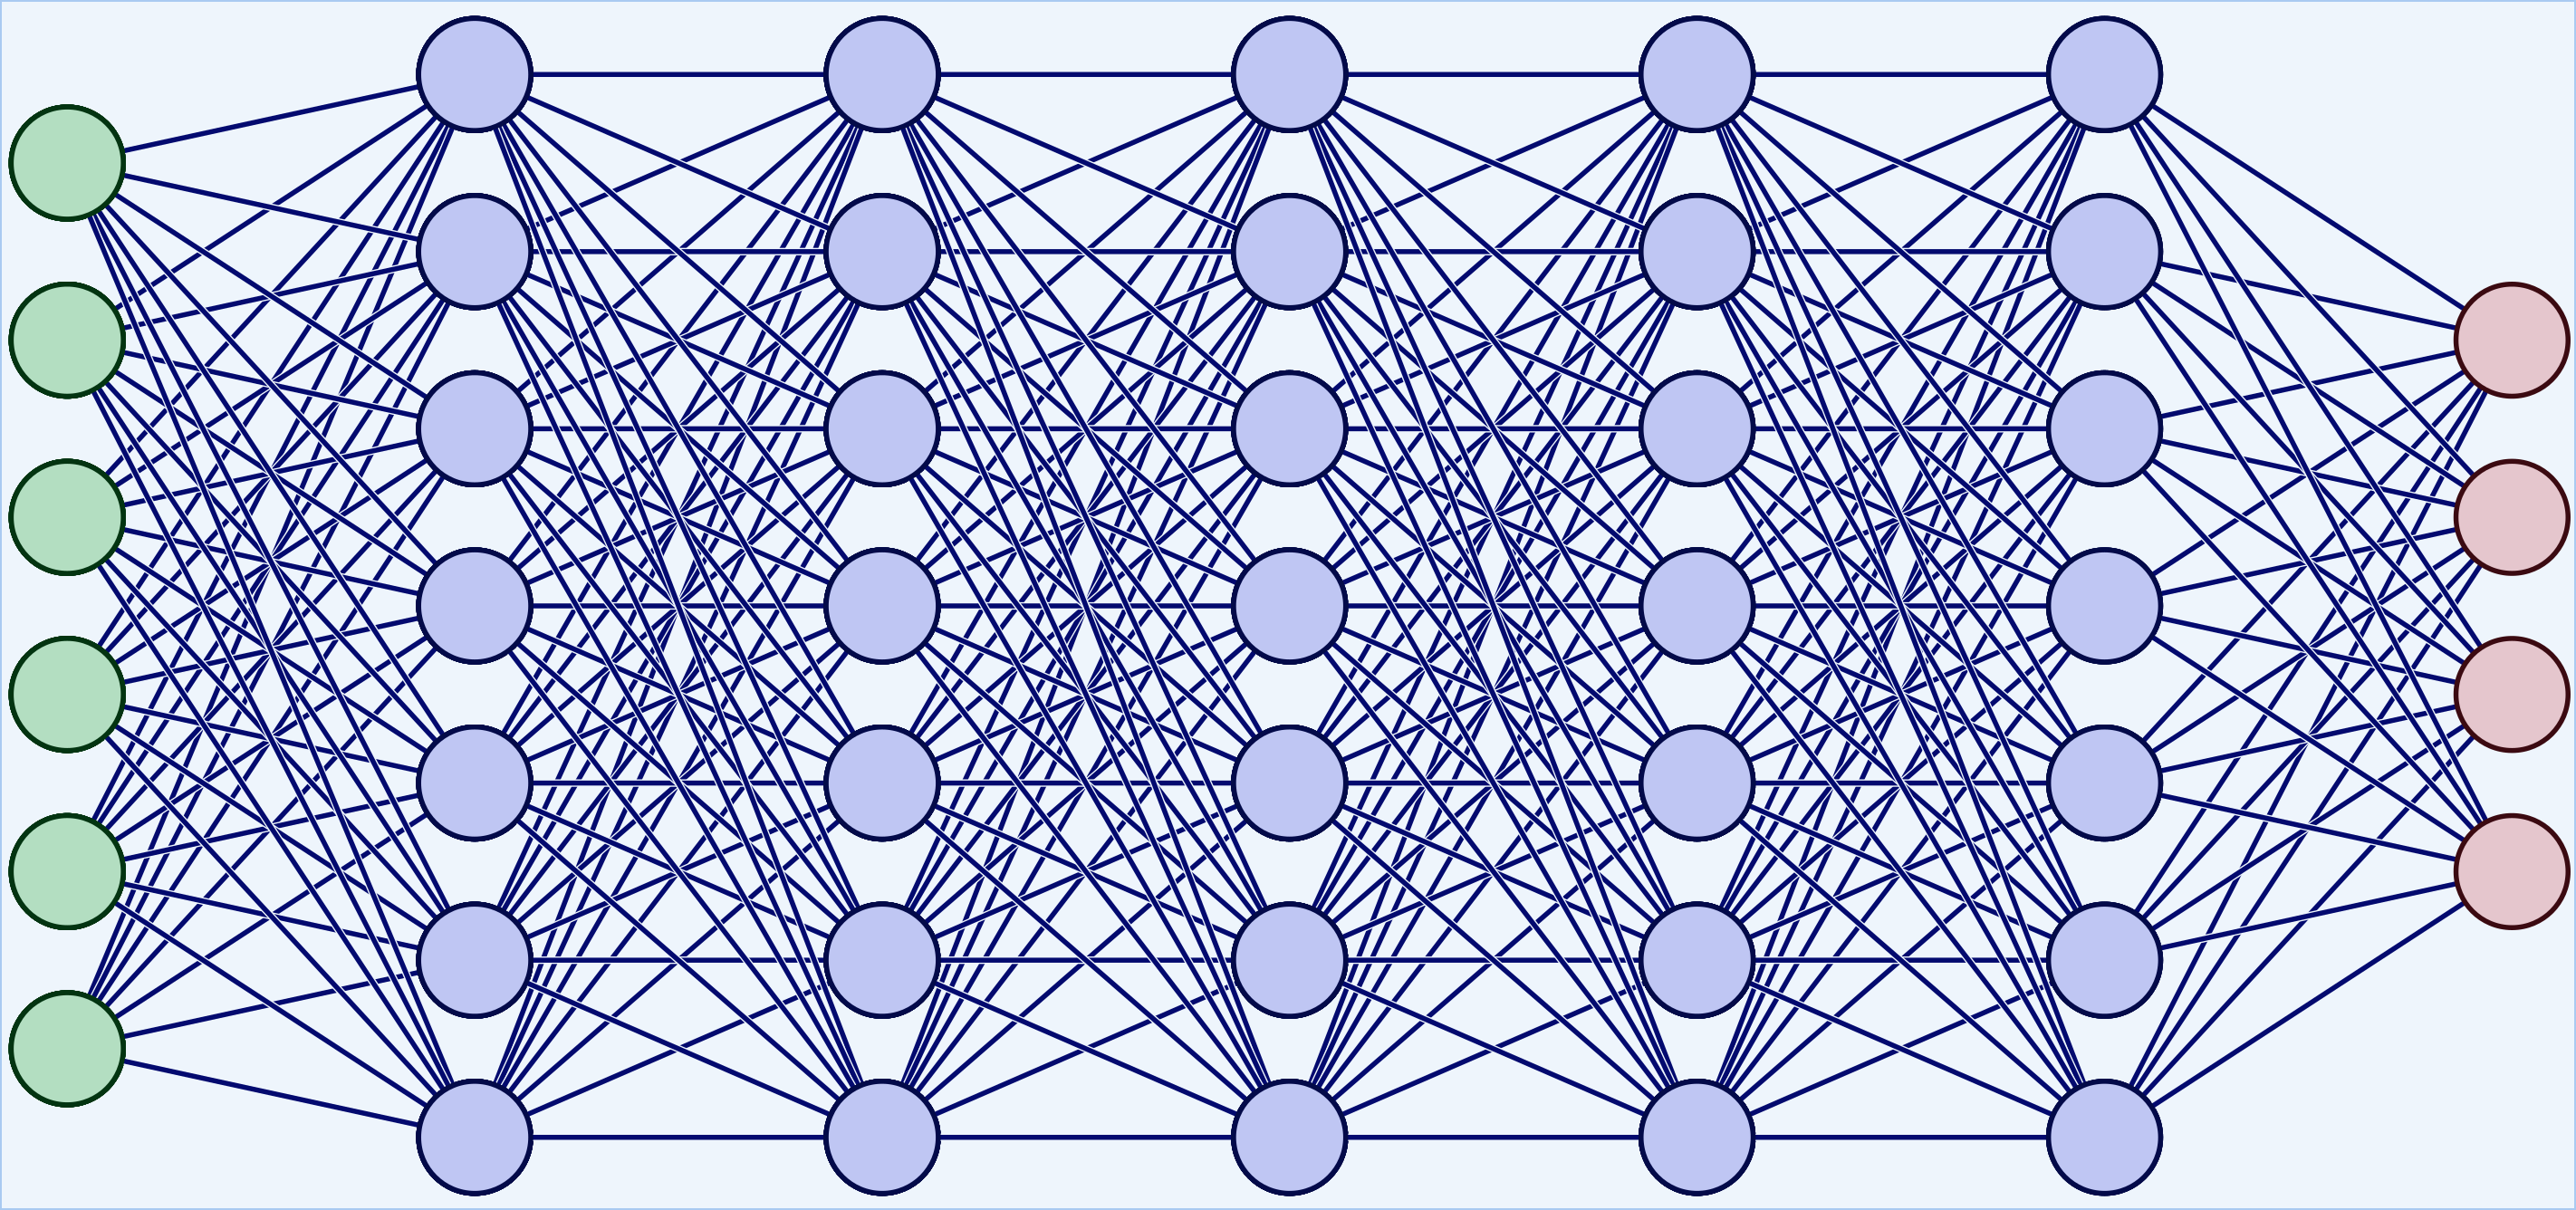
\includegraphics[width=0.52\linewidth]{deep-NN}
  \end{flushright}
  \vspace{-0.7em}
  {\large\textbf{Definición}}:\par
  una \structure{\bf Red Neuronal} (\textit{RN} o \textit{NN}) es una función $f_{NN}:\Rset^n \to \Rset^m$ del tipo:
    $$
    {\color{outcolor}\mathbf{y}} = f_{NN}({\color{inputcolor}x}) = 
    {\color{hiddencolor} \ff_L\circ \cdots \circ \ff_2\circ \ff_1({\color{inputcolor} x})}.
    $$
  Donde...
  \begin{itemize}\itemsep=0.5em
    \item Cada función $\ff_i$ se llama una \textbf{capa} (
      {\color{inputcolor}entrada} $\rightarrow$
      {\color{hiddencolor}oculta} $\rightarrow$ 
      {\color{outcolor}salida} )
    \item Cada capa $\ff_i$ está compuesta por un nº variable de \textbf{neuronas}
    \item Cada neurona depende un conjunto de \textbf{parámetros}, que determinarán a la RN 
  \end{itemize} 
  \bigskip
  \scriptsize
  \begin{flushright}
  $\star$ La RN de la figura  se dice de tipo «\textit{feed forward}» o {prealimentada}
  \end{flushright}
\end{frame}

\begin{frame}{Un ejemplo}
  \vspace{-0.5em}
  \begin{center}
  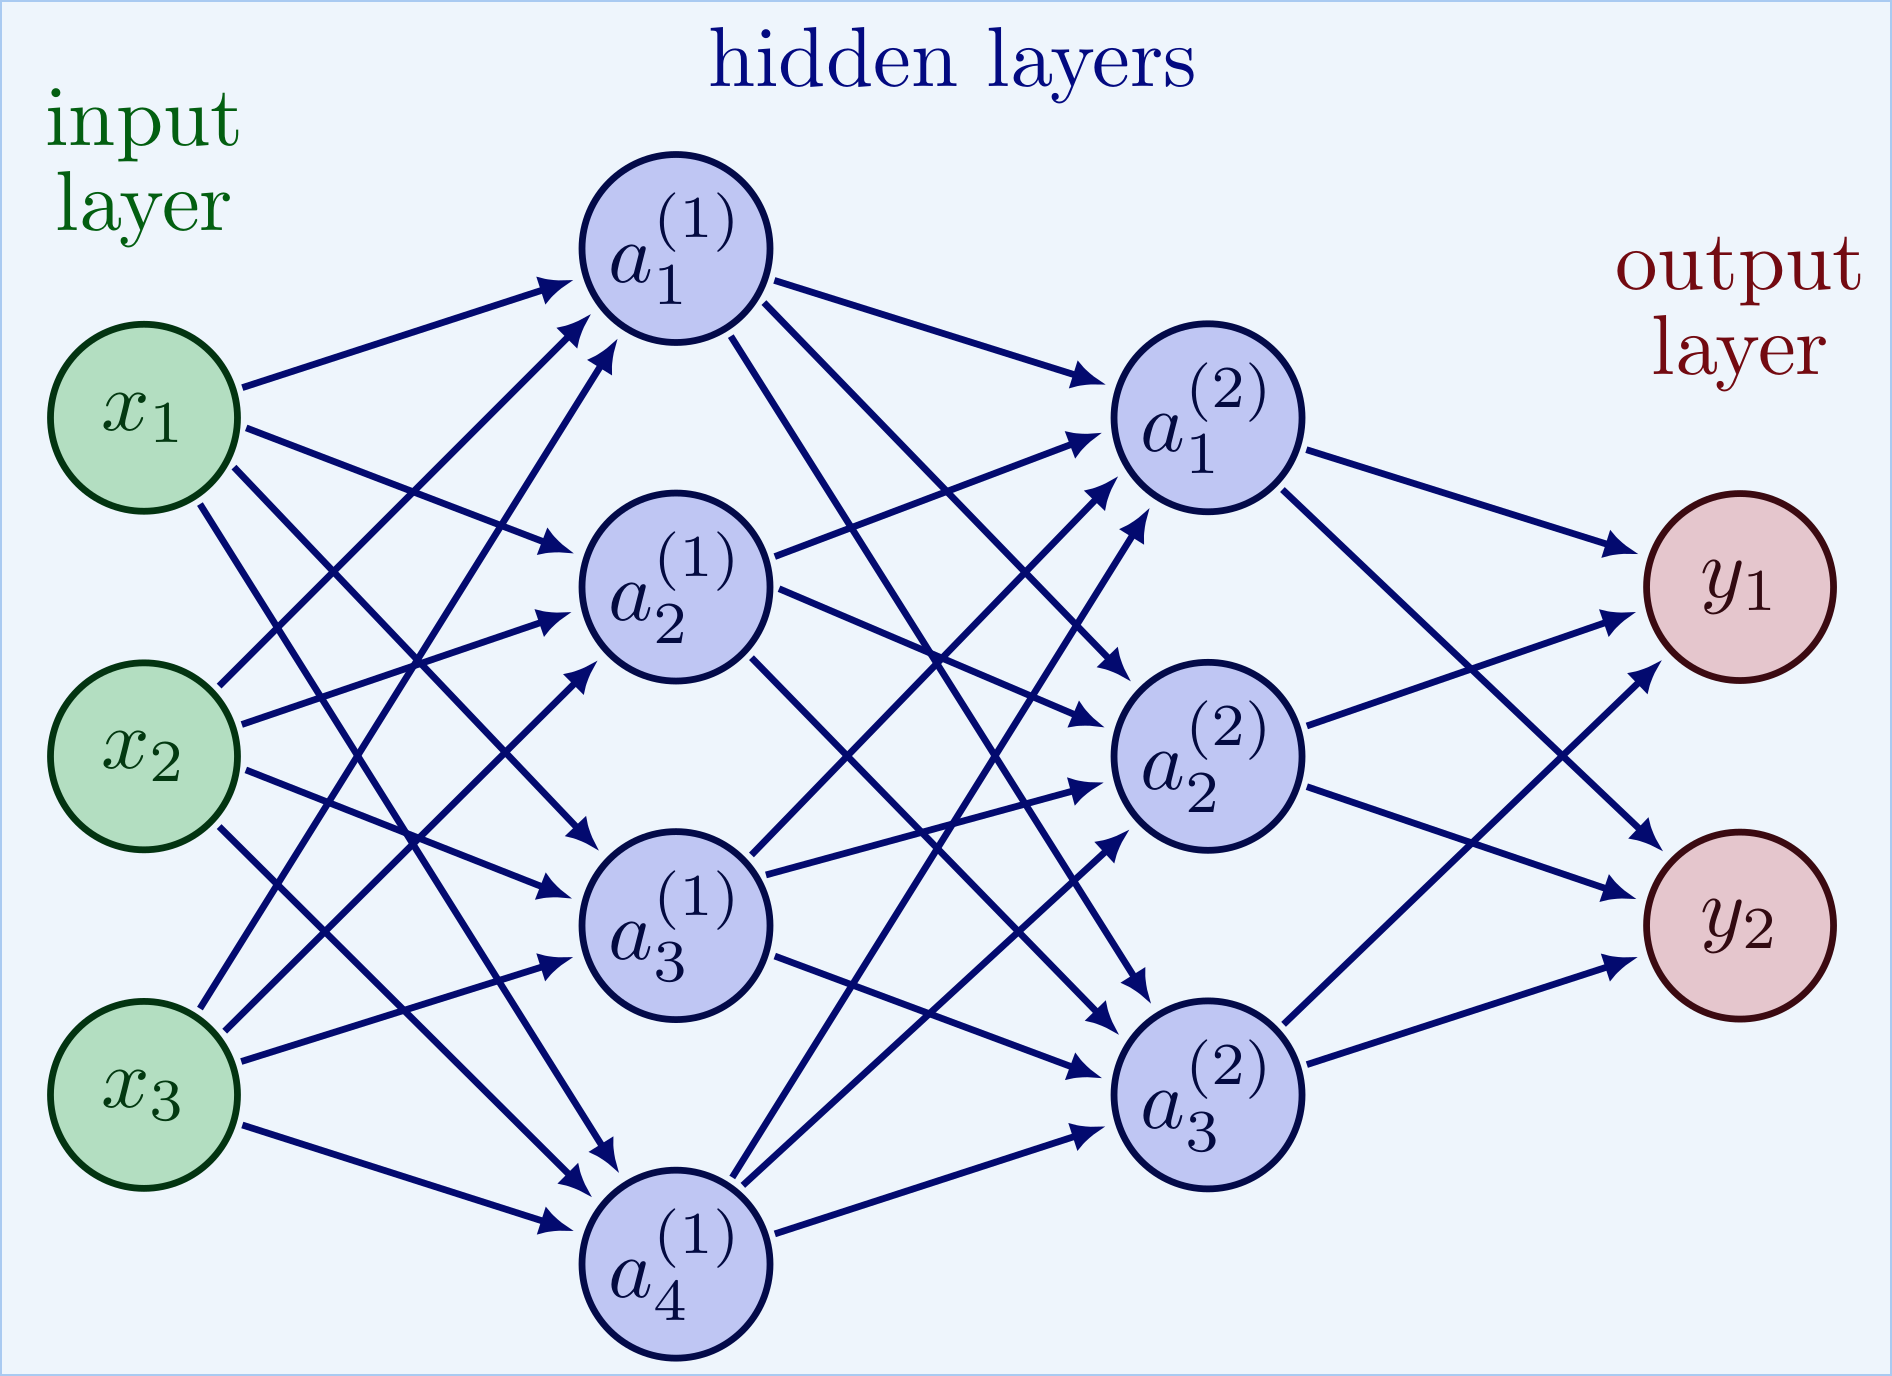
\includegraphics[width=0.82\linewidth]{example-NN}
  \end{center}
  $$
  f_{NN}:\Rset^3 \to \Rset^2
  \mbox{con $2$ capas ocultas de $4$ y $3$ neuronas}
  $$
\end{frame}


\begin{frame}{Neurona o \emph{perceptrón} simple}
  Cada neurona $j$ de una capa oculta $f_i$ (o de salida $y_i$) es una función% 
  \footnote{Donde $N_i$ es el número de neuronas de la capa $i-1$}:
  $$
  \xx\in \Rset^{N_{i}} \rightarrow \alert{a_j^{(i)}}(\xx) \in \Rset,
  $$
  composición de%
  \begin{itemize}
    \item una función afín con parámetros $\structure{\ww}=({w_1},\dots,{w_{N_i}})$ y \structure{$b$}
    \item una función no lineal $\sigma$, llamada «\structure{función de activación}»  
  \end{itemize}
  \begin{block}{}
    \vspace{-0.8em}
  \begin{align*}
    \alert{a_j^{(i)}}(\xx) &= \sigma(w_1 x_1 + w_2 x_2 + \cdots + w_{N_i} x_{N_i} + b) = \\
                   &=\sigma\Big(\sum_{k=1}^{N_i} w_k x_k +b\Big) = \sigma(\ww\cdot\xx + b)
  \end{align*}
  \end{block}
\end{frame}

\begin{frame}{Con más propiedad...}
Para aligerar la notación se omitieron los índices correspondientes a la capa, $i$, y a la neurona, $j$. Debería ser:
  \begin{align*}
    \alert{a_j^{(i)}}(\xx) = \sigma\Big(\sum_{k=1}^{N_i} w^{(i)}_{j,k} x_k +b^{(i)}_j\Big).
    % = \sigma\big(\ww^{(i)}\cdot\xx + b^{(i)}_j\big)
  \end{align*}
  Así, si $\WW^{(i)}$ denota a la matriz de valores $w^{(i)}_{j,k}$, y $\vect b^{(i)}$ es el vector $(b^{(i)}_j)$, podemos escribir a tod la \alert{capa} $i$ como:
$$
\alert{\ff_i(\xx)} = {\boldsymbol\sigma_i}(\WW^{(i)}\xx + \vect b^{(i)})
$$
La RN está determinada por los parámetros $\WW^{(i)}$, los desplazamientos $\vect b^{(i)}$ y las funciones de activación $\boldsymbol\sigma_i$
\end{frame}

\section{Partes básicas de una red neuronal}

%\alert{descenso de gradiente}\footnote{\url{https://en.wikipedia.org/wiki/Gradient_descent}}
\begin{frame}{Funciones de activación}
Es una abstración que representa la \structure{\bf tasa potencial de acción.}
\begin{center}
  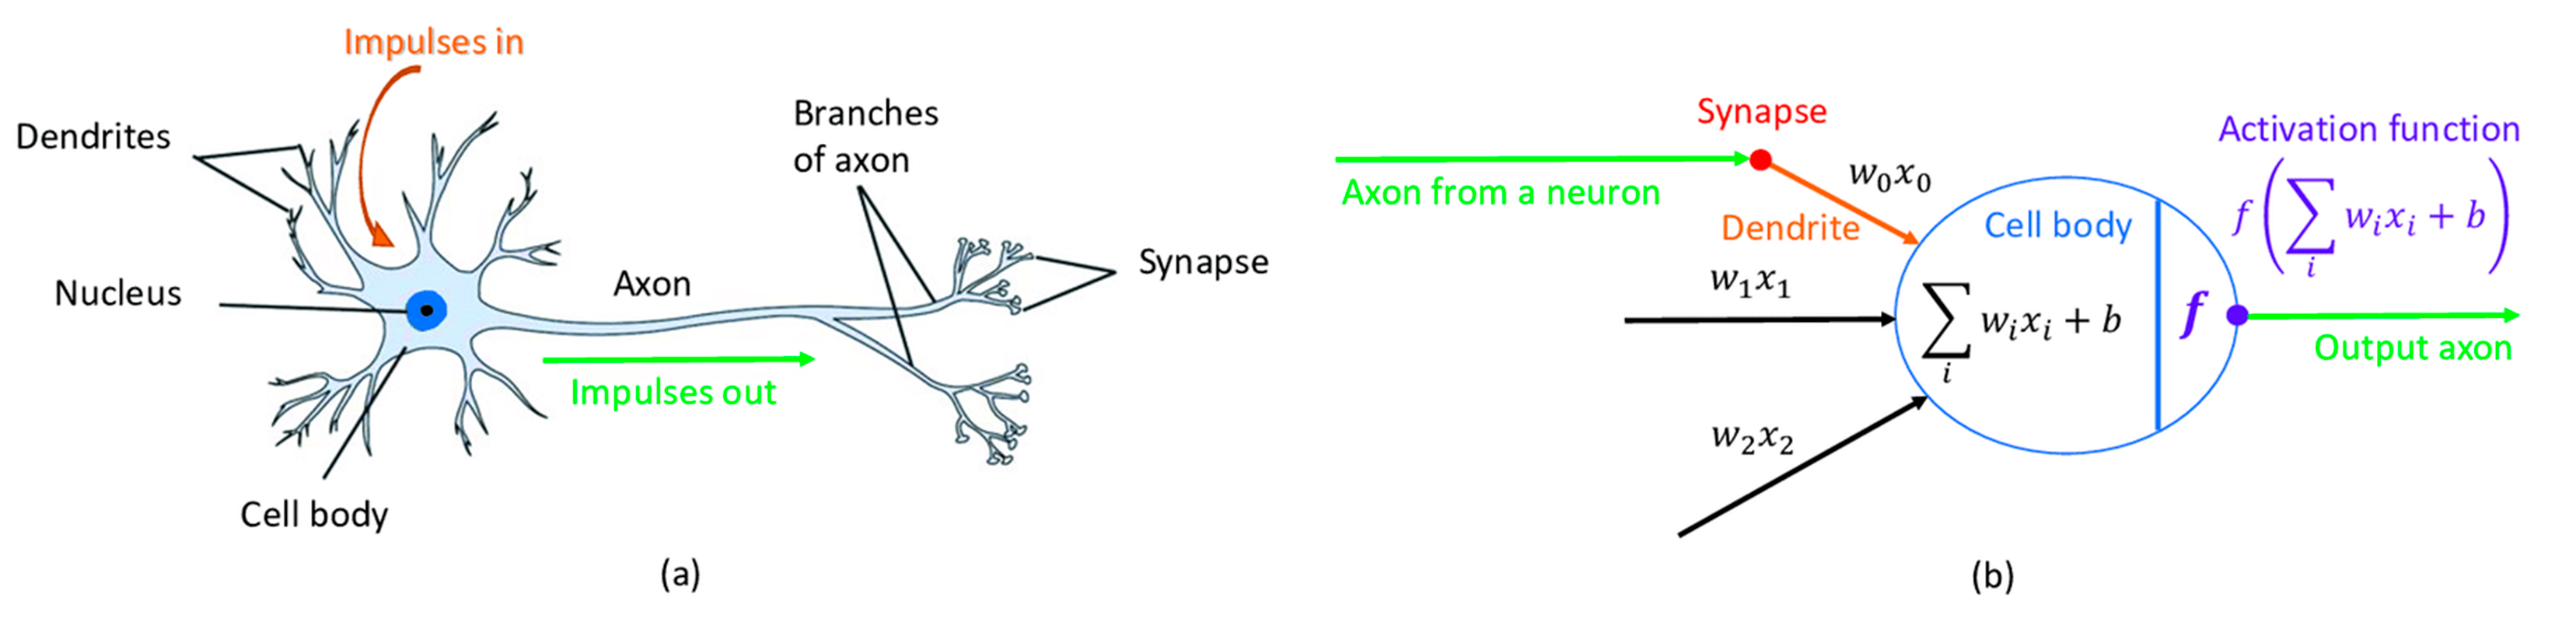
\includegraphics[width=1\linewidth]{src/Activation-IMG-1.png}
  \footnote{\href{https://www.researchgate.net/publication/317679065_Ranking_to_Learn_and_Learning_to_Rank_On_the_Role_of_Ranking_in_Pattern_Recognition_Applications}{Ranking to Learn and Learning to Rank: On the Role of Ranking in Pattern Recognition Applications}}
\end{center}
Dada una entrada se procesa \textbf{(parte lineal)} y se valora si la neurona dispara o no \alert{perceptron}. Para comportamientos más complejos podemos devolver una probabilidad
si es baja menos probable es que dispare y viceversa, de ahí proviene la \alert{función de activación sigmoidal.}
\end{frame}

\begin{frame}{¿Por qué necesitamos funciones de activación?}
  Supongamos que no tenemos funciones de activación, luego la red neural es composición de aplicaciones lineales, esto implica que \structure{\bf la
  red es una función lineal.}
  $$f_{NN}({\color{inputcolor}x}) = {\color{hiddencolor}w_1 x_1 + w_2 x_2 + \cdots + w_{N_i} x_{N_i} + b}$$
  Por lo tanto, no importa cuantas capas tenga el modelo, puesto que estamos realizando una transformación lineal en las entradas.
  Esto es un problema, puesto que no podemos \alert{modelar problemas no lineales}.

  % Ejemplo de problemas no lineales y lineales por ejemplo de ajustar ecuaciones o similar.

\end{frame}

\begin{frame}{Representación de funciones de activación}
  \vspace{-0.7em}
  \begin{center}
  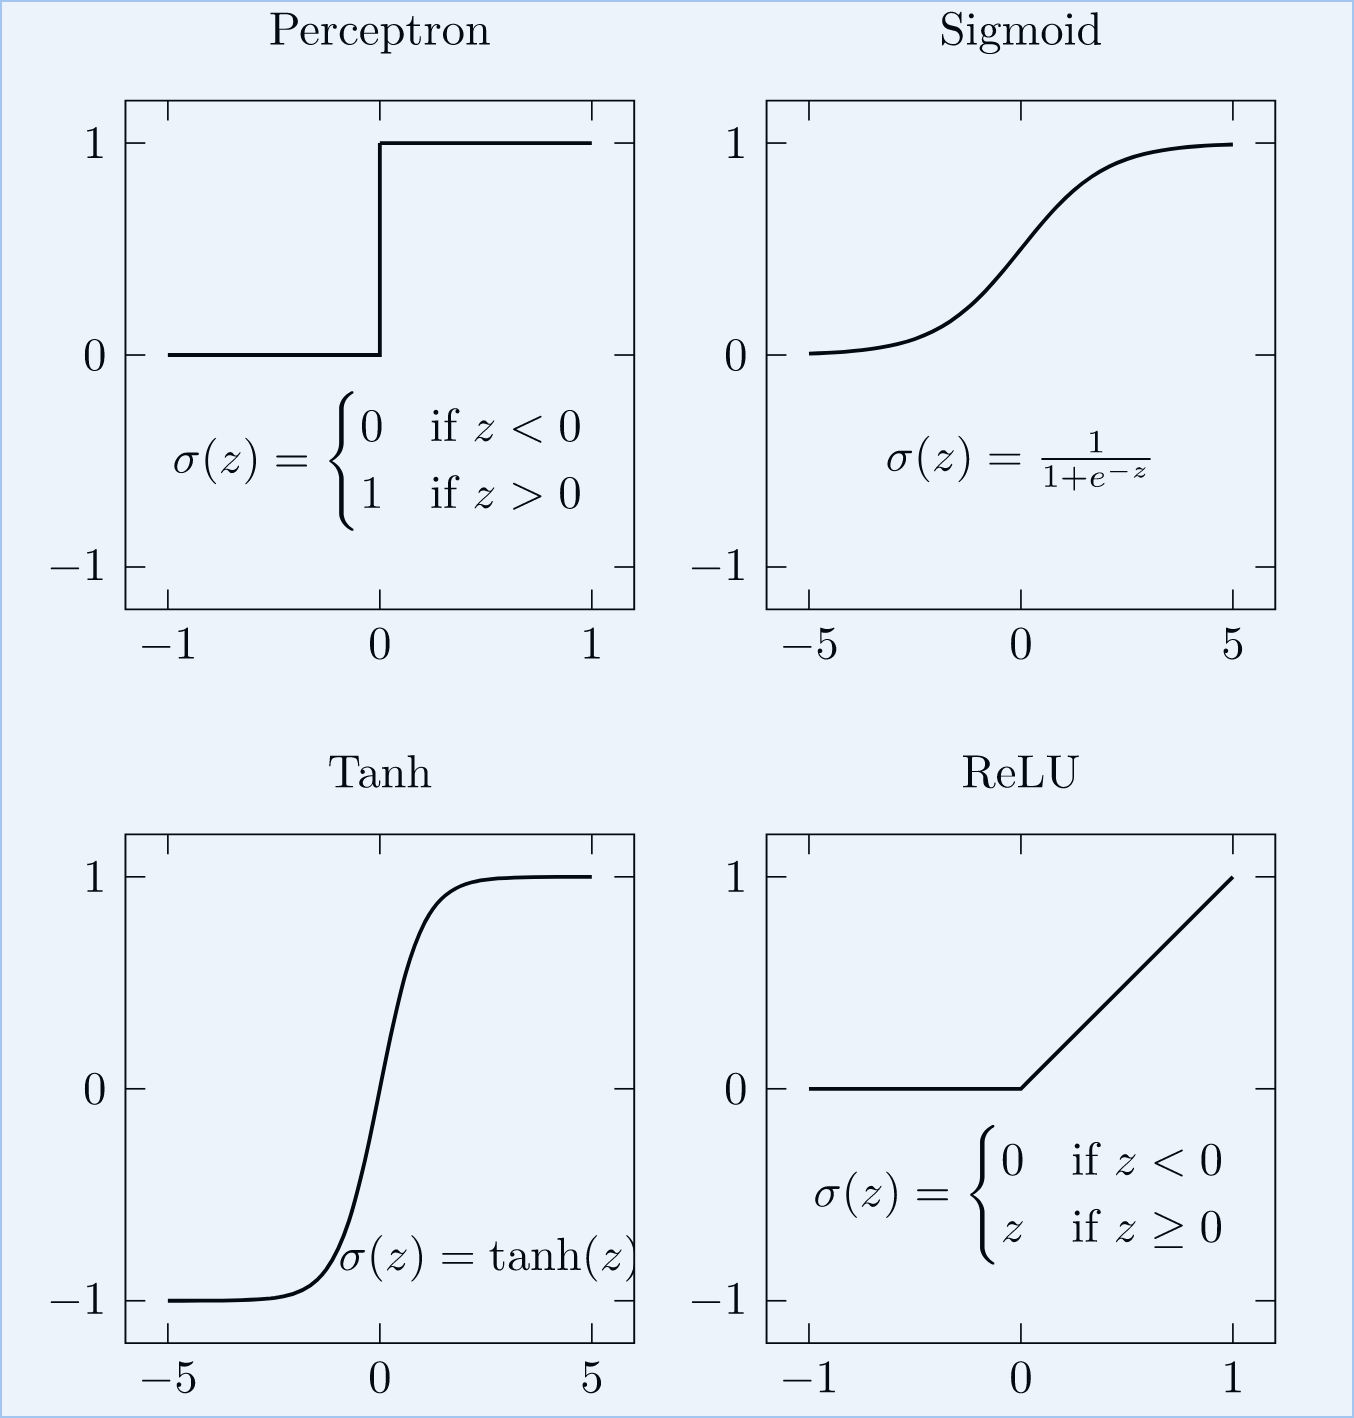
\includegraphics[width=0.65\linewidth]{funciones_activacion}
  \end{center}
\end{frame}

\begin{frame}{Funciones de perdida}
Una función de perdida compara la salida de la red neuronal con la salida esperada, y nos dice que tan \structure{\bf bien o mal lo esta haciendo la red neuronal.}

\vspace*{0.8em}

Cuando entrenamos, nuestro objetivo es \alert{minimazar la perdida entre la salida esperada y la salida de la red neuronal.}

\vspace*{0.8em}

Ejemplos:
\begin{itemize}
  \item Problema de regresión $$
  y_{pred}=\begin{pmatrix}
    250 & 300 \\
    300 & 400 \\ 
  \end{pmatrix}
  \hspace*{0.8em}
  y_{real} = \begin{pmatrix}
    100 & 150 \\
    400 & 200 \\
  \end{pmatrix}
  $$
  \item Problema de clasificación
  $$
  y_{pred}=\begin{bmatrix}
    0.12 \\
    0.48 \\
    0.4 \\ 
  \end{bmatrix}
  \hspace*{0.8em}
  y_{real} = \begin{bmatrix}
    0 \\
    1 \\
    0 \\
  \end{bmatrix}
  $$
\end{itemize}
\end{frame}

\begin{frame}
  Podemos pensarlo como un residuo en estadística, que se encarga de  medir la distancia entre los \textbf{valores actuales de y y los de la linea de regresión} (valores predecidos).
  
  \vspace{0.8em}

  \textbf{El objetivo es minimizar la distancia neta.}
  \begin{center}
    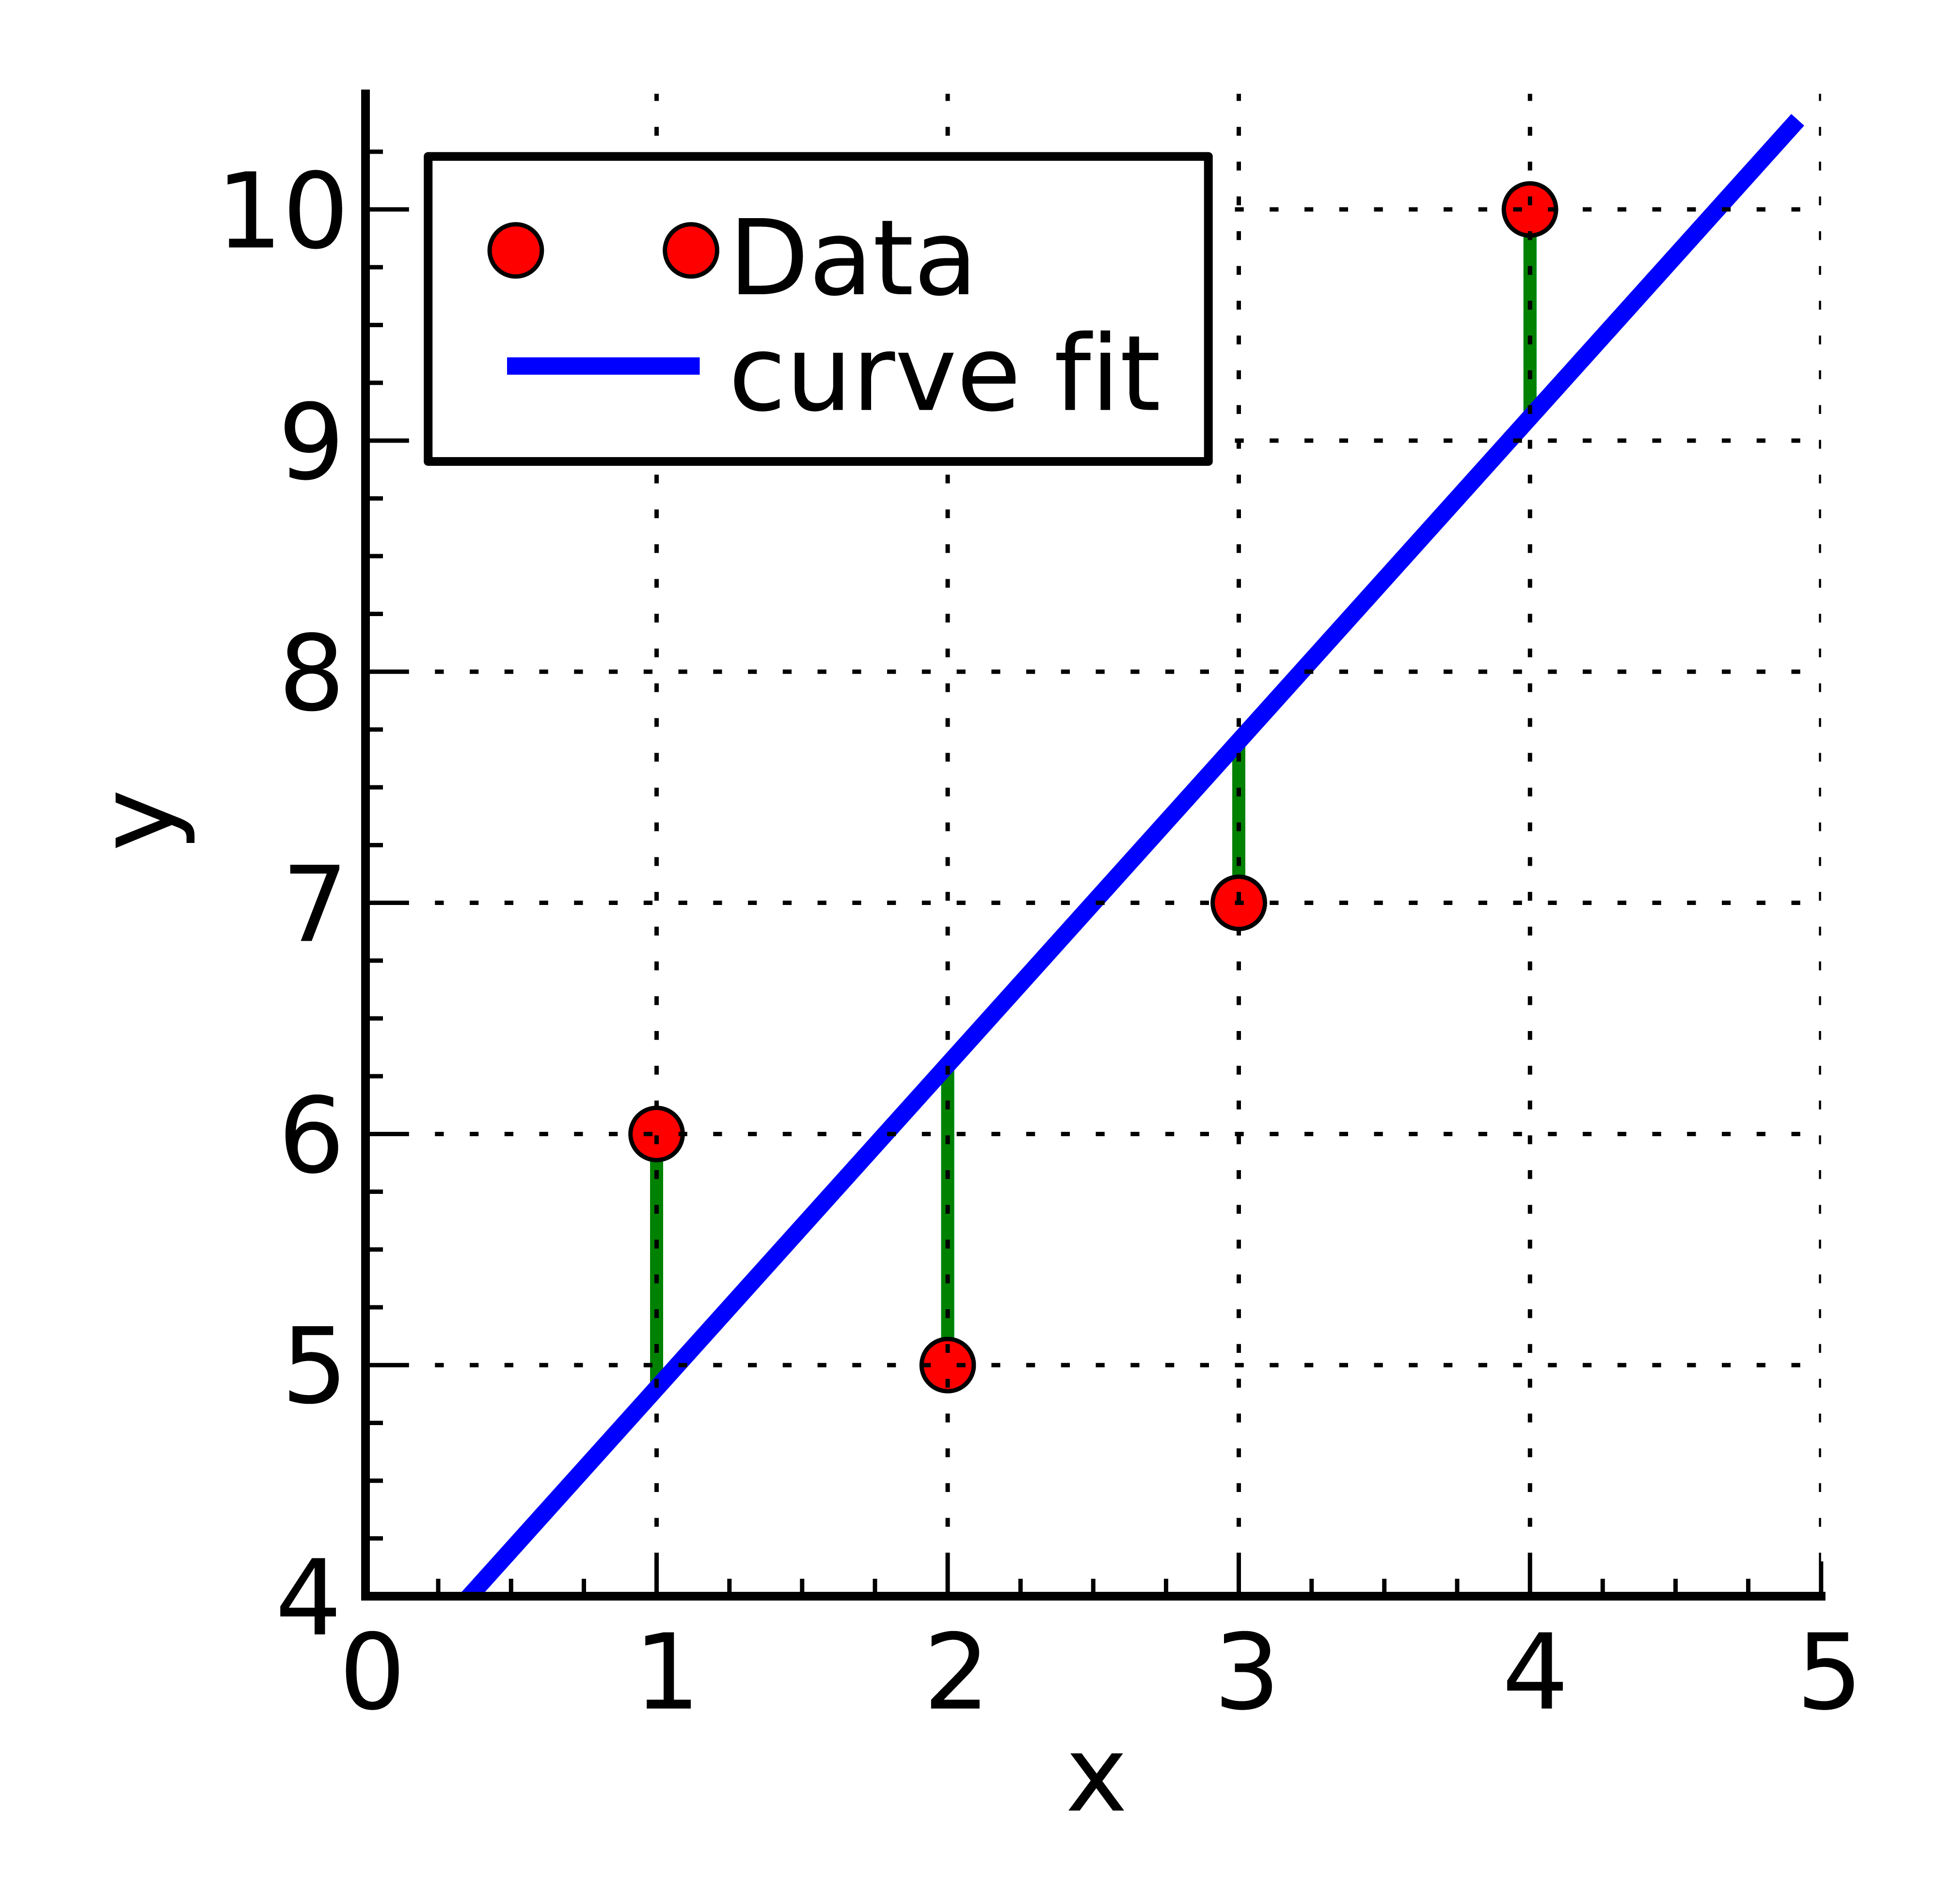
\includegraphics[width=0.5\linewidth]{src/Linear_regression.png}
    \footnote{\href{https://en.wikipedia.org/wiki/Linear_regression}{Wikipedia - Linear regression}}
  \end{center}
  % Añadir ejemplo estadística
\end{frame}

\begin{frame}{Ejemplos de funciones de perdida}
Principalmente se agrupan en:
\begin{itemize}
  \item \structure{\bf Perdida de regresión:} Dado un valor de entrada, el modelo predice el valor de salida. 
  
  \vspace{0.5em}

  Ejemplos: \textbf{Mean Squared Error, Mean Absolute Error...}

  $$MSE=\frac{1}{n}\sum_{i=1}^{n}(y^{(i)} - y_{pred}^{(i)})^2 $$
  $$MAE=\frac{1}{n}\sum_{i=1}^{n}| y^{(i)} - y_{pred}^{(i)}| $$
  \item \structure{\bf Perdida de clasificación:} Dado un valor de entrada, el modelo devuelve un vector de probabilidades de que la entrada pertencezca a una serie de categorias preestablecidas.

  \vspace{0.5em}

  Ejemplos: \textbf{Binary Cross Entropy, Categorical Cross Entropy...}

\end{itemize}
\end{frame}

\begin{frame}{Optimizadores}
Son algoritmos que se usan para \structure{\bf minimizar la función de perdida} o maximizar la función de ganancia.
Ejemplos: \alert{Adam, RMSprop, SGD...}
\vspace*{0.8em}

Cada vez que predecimos un valor mediante la red y comparamos con el valor real, \textbf{el optimizador ajusta los pesos de la red para minimizar la perdida.}
\begin{center}
  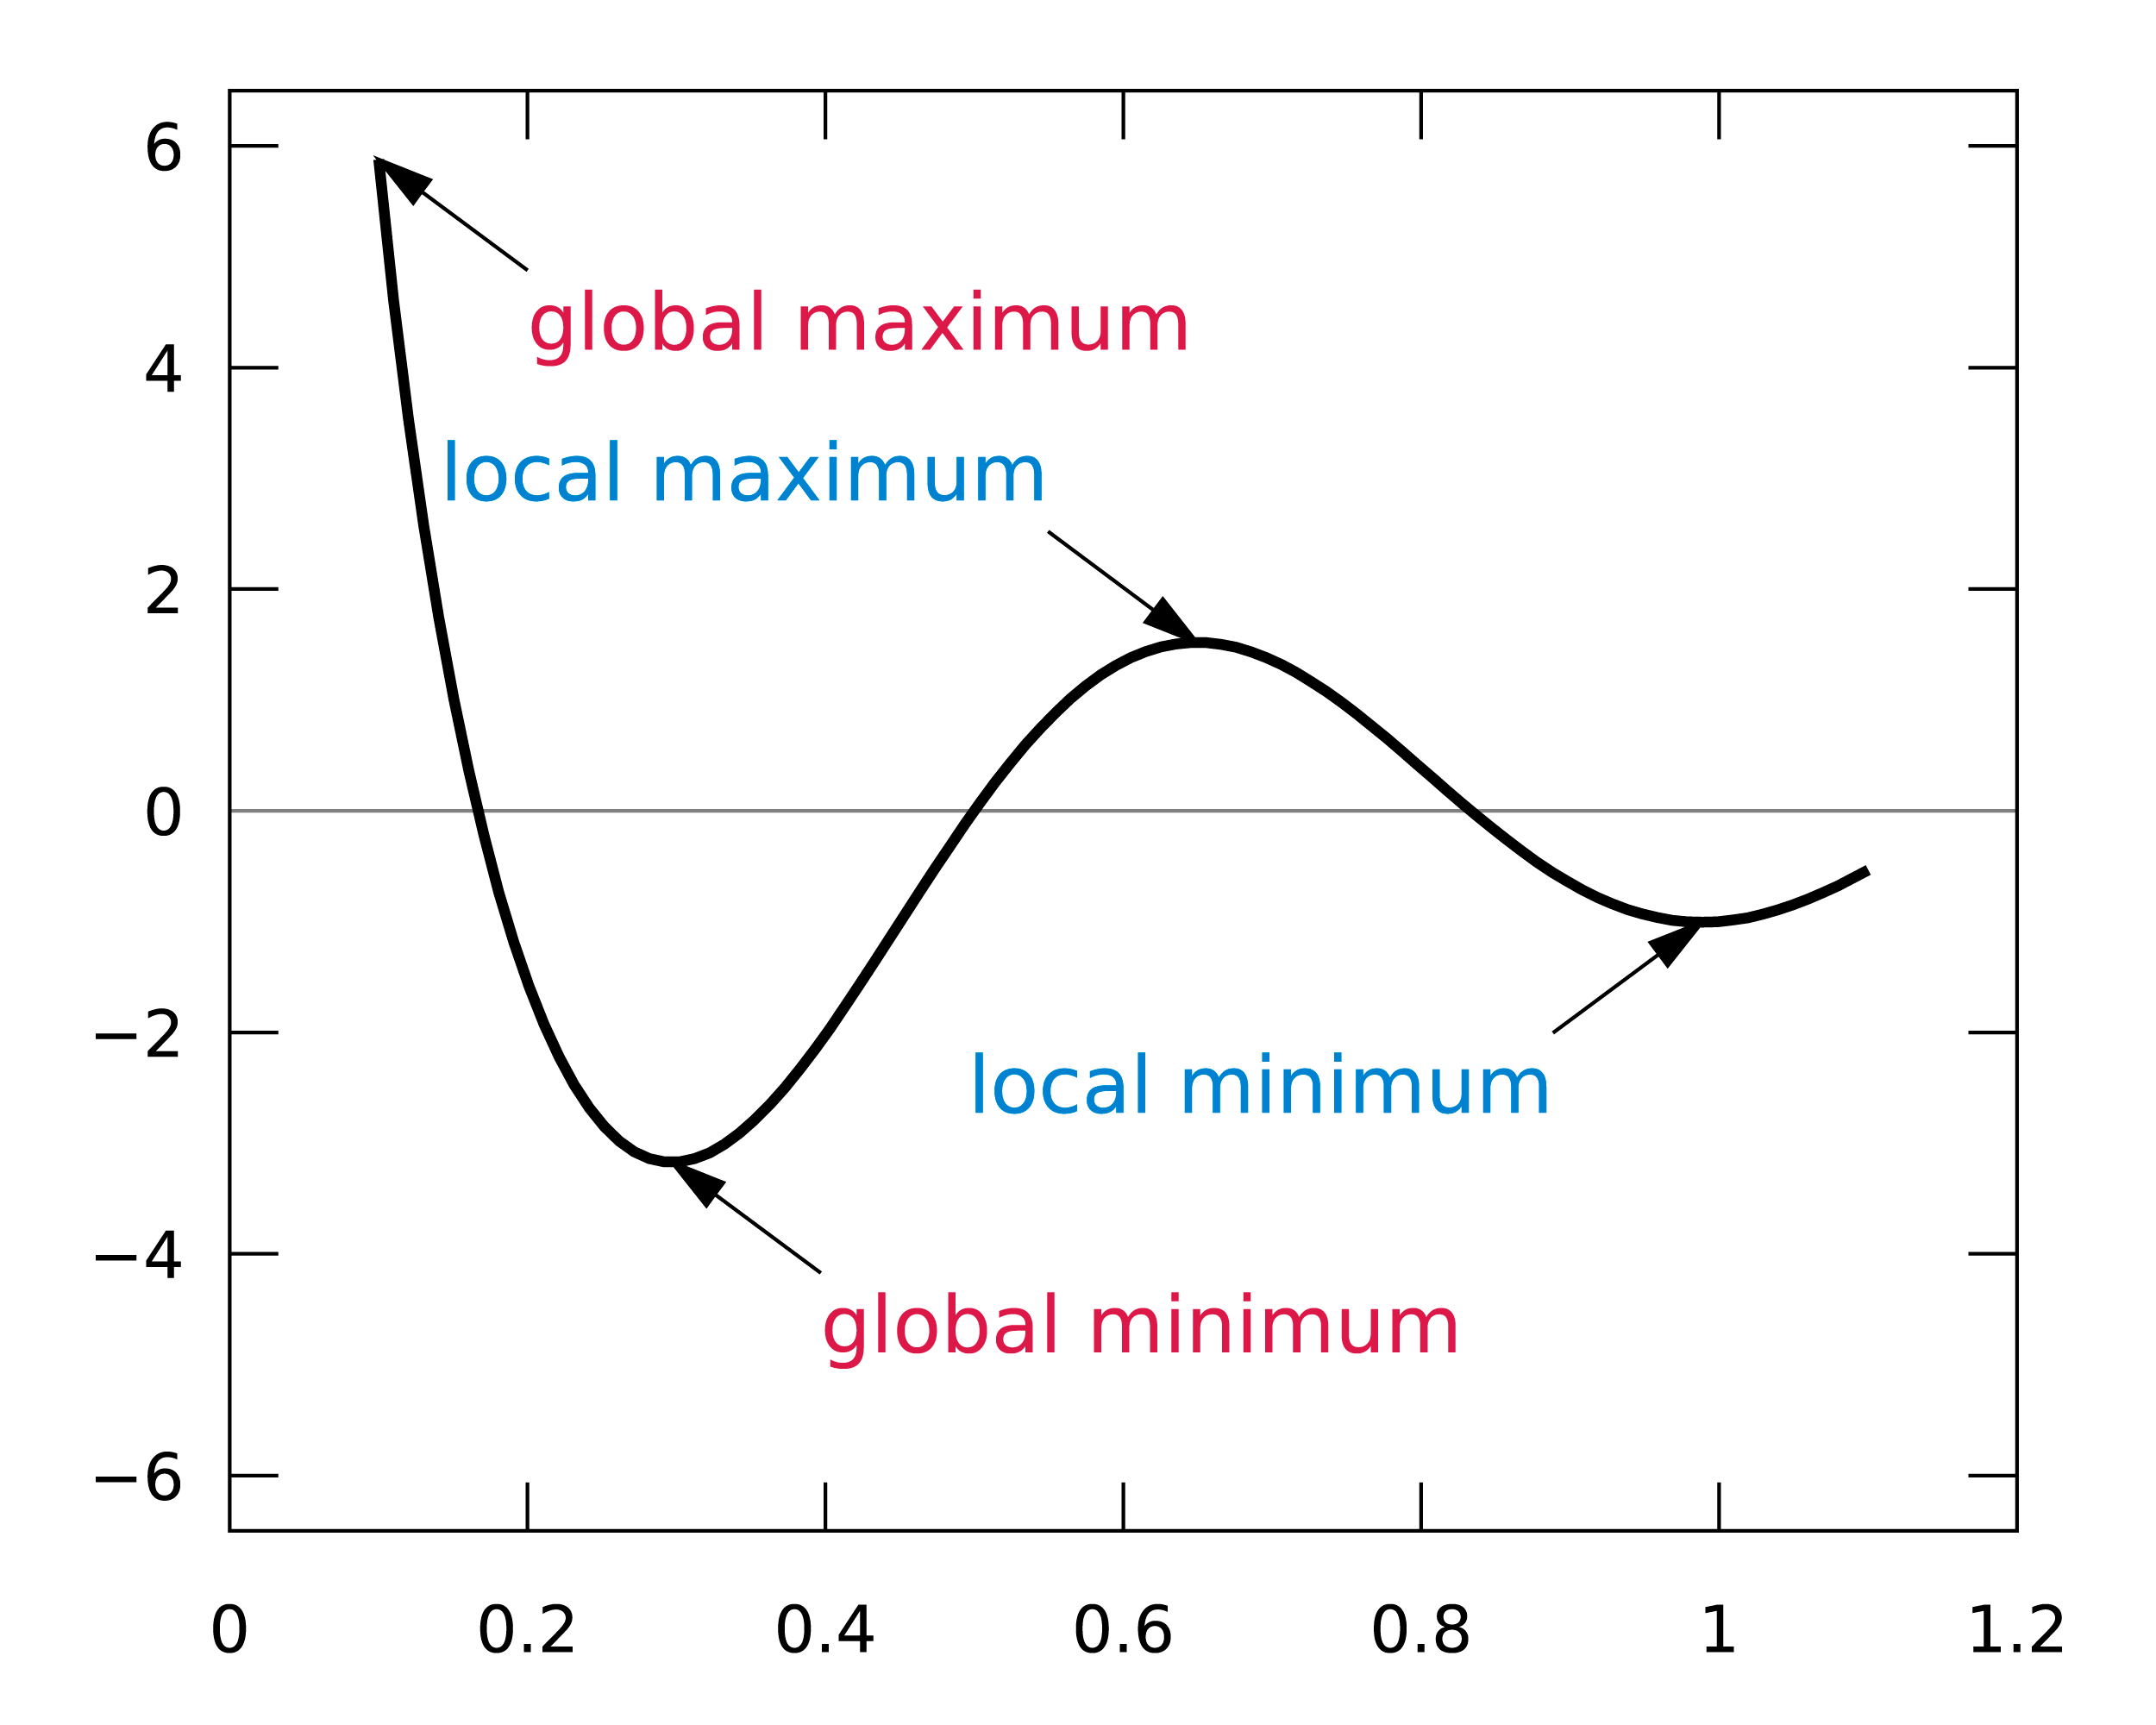
\includegraphics[width=0.4\linewidth]{src/Extrema_example_original.png}
\end{center}
Queremos obtener un mínimo global en la función de perdida. 



\end{frame}

\begin{frame}{Gradient Descent\footnote{\href{https://tiranex.github.io/Gradient-Descent/}{Simulador de descenso de gradiente - Elaboración Propia}}}
El algoritmo de descenso de gradiente es un \structure{\bf algoritmo de optimización que se utiliza para minimizar una función objetivo.}


Para implementarlo:
$$a_{n+1}=a_n - \delta \nabla F(a_n)$$

La idea es que el gradiente muestra la dirección de descenso entonces al movernos en esa dirección vamos a llegar a un mínimo, el problema es que puede no ser un mínimo global.
% Añadir ejemplo imagen
% Añadir ejemplo web
\end{frame}

\begin{frame}{¿Cómo se calculan las derivadas?}
Se emplea una técnica llamada \structure{\bf Backpropagation} que se encarga de calcular las derivadas de la función de perdida con respecto a los pesos de la red.

\vspace{0.8em}

Ejemplo: \alert{$f(x,y)=(\frac{x}{y}+5)^2+x$ \hspace{0.8em}$\frac{\partial f}{x}(6,2)$}

\vspace{0.8em}

Construimos el grafo de computación:

$$
\begin{array}{|c|c|} \hline
  w_0=x                                                            \\ \hline
  w_1=y                                                                        \\ \hline
  w_2=w_0/w_1+5              \\ \hline
  w_3=w_2^2                    \\ \hline
  w_4=w_3+w_0                \\ \hline
\end{array}
$$
\end{frame}

\begin{frame}{¿Cómo se calculan las derivadas?}
  Se emplea una técnica llamada \structure{\bf Backpropagation} que se encarga de calcular las derivadas de la función de perdida con respecto a los pesos de la red.
  
  \vspace{0.8em}
  
  Ejemplo: \alert{$f(x,y)=(\frac{x}{y}+5)^2+x$ \hspace{0.8em}$\frac{\partial f}{x}(6,2)$}
  
  \vspace{0.8em}
  
  Hacemos un pasada evaluando cada nodo.
  
  $$
  \begin{array}{|c|c|} \hline
    w_0=x              & w_0=6                                             \\ \hline
    w_1=y                     & w_1 = 2                                                   \\ \hline
    w_2=w_0/w_1+5           & w_2=8   \\ \hline
    w_3=w_2^2           &w_3=64         \\ \hline
    w_4=w_3+w_0          &w_4=70      \\ \hline
    \end{array}
  $$
\end{frame}

\begin{frame}{¿Cómo se calculan las derivadas?}
  Se emplea una técnica llamada \structure{\bf Backpropagation} que se encarga de calcular las derivadas de la función de perdida con respecto a los pesos de la red.
  
  \vspace{0.8em}
  
  Ejemplo: \alert{$f(x,y)=(\frac{x}{y}+5)^2+x$ \hspace{0.8em}$\frac{\partial f}{x}(6,2)$}
  
  \vspace{0.8em}
  
  Empleamos la regla de la cadena en reverso.
  
  $$
  \begin{array}{|c|c|c|} \hline
    w_0=x              & w_0=6    & \frac{\partial z}{\partial w_0}=\frac{\partial z}{\partial w_2}\frac{\partial w_2}{\partial w_0} + \frac{\partial z}{\partial w_4}\frac{\partial w_4}{\partial w_0} = (2\cdot w_2)\cdot \frac{1}{w_1}+1                                       \\ \hline
    w_1=y                     & w_1 = 2 & \frac{\partial z}{\partial w_1}=\frac{\partial z}{\partial w_2}\frac{\partial w_2}{\partial w_1}                          =2\cdot w_2 \cdot(\frac{-w_0}{w_1^2})                        \\ \hline
    w_2=w_0/w_1+5           & w_2=8 & \frac{\partial z}{\partial w_2}=\frac{\partial z}{\partial w_3}\frac{\partial w_3}{\partial w_2}=2\cdot w_2   \\ \hline
    w_3=w_2^2           &w_3=64        & \frac{\partial z}{\partial w_3}=\frac{\partial z }{\partial w_4}\frac{\partial w_4}{\partial w_3}=1 \\ \hline
    w_4=w_3+w_0          &w_4=70 & \frac{\partial z}{\partial w_4}=1 (seed)      \\ \hline
    \end{array}
  $$
\end{frame}

\begin{frame}{¿Cómo se calculan las derivadas?}
  Se emplea una técnica llamada \structure{\bf Backpropagation} que se encarga de calcular las derivadas de la función de perdida con respecto a los pesos de la red.
  
  \vspace{0.8em}
  
  Ejemplo: \alert{$f(x,y)=(\frac{x}{y}+5)^2+x$ \hspace{0.8em}$\frac{\partial f}{x}(6,2)$}
  
  \vspace{0.8em}
  
  Sustituyendo obtenemos $\frac{\partial f}{x}(6,2)= 9$ $\frac{\partial f}{y}(6,2)=-24$
  
  $$
  \begin{array}{|c|c|c|} \hline
    w_0=x              & w_0=6    & \frac{\partial z}{\partial w_0}=9                                      \\ \hline
    w_1=y                     & w_1 = 2 & \frac{\partial z}{\partial w_1}=-24                        \\ \hline
    w_2=w_0/w_1+5           & w_2=8 & \frac{\partial z}{\partial w_2}=16   \\ \hline
    w_3=w_2^2           &w_3=64        & \frac{\partial z}{\partial w_3}=1 \\ \hline
    w_4=w_3+w_0          &w_4=70 & \frac{\partial z}{\partial w_4}=1 (seed)      \\ \hline
    \end{array}
  $$
\end{frame}

\begin{frame}{Hiperparámetros}
  Un hiperparámetro es un \structure{\bf valor constante que se establece previo al  entrenamiento.}
  
  \vspace*{0.8em}
  
  Ejemplos: \alert{Tasa de aprendizaje, número de capas, funciones de activación, funciones de perdida, optimizadores...}

  \vspace*{0.8em}

  Si un modelo no se comporta bien, entonces tenemos que modificar los hiperparámetros, ya sea para conseguir que la red aprenda más lento (tasa de aprendizaje), hacerlo más complejo (añadir más capas)\dots
\end{frame}
\begin{frame}{Tasa de aprendizaje}
  La tasa de aprendizaje define el \structure{\bf tamaño de los pasos correctivos para que el modelo ajuste los errores en cada observación.} 
  \begin{itemize}
    \item \alert{Tasa de aprendizaje alta} $\rightarrow$ 
    

    Tiempo de entrenamiento menor $//$ Precisión menor
    \item \alert{Tasa de aprendizaje baja} $\rightarrow$ 
    
    
    Tiempo de entrenamiento mayor $//$ Precisión mayor
  \end{itemize}
  \begin{center}
    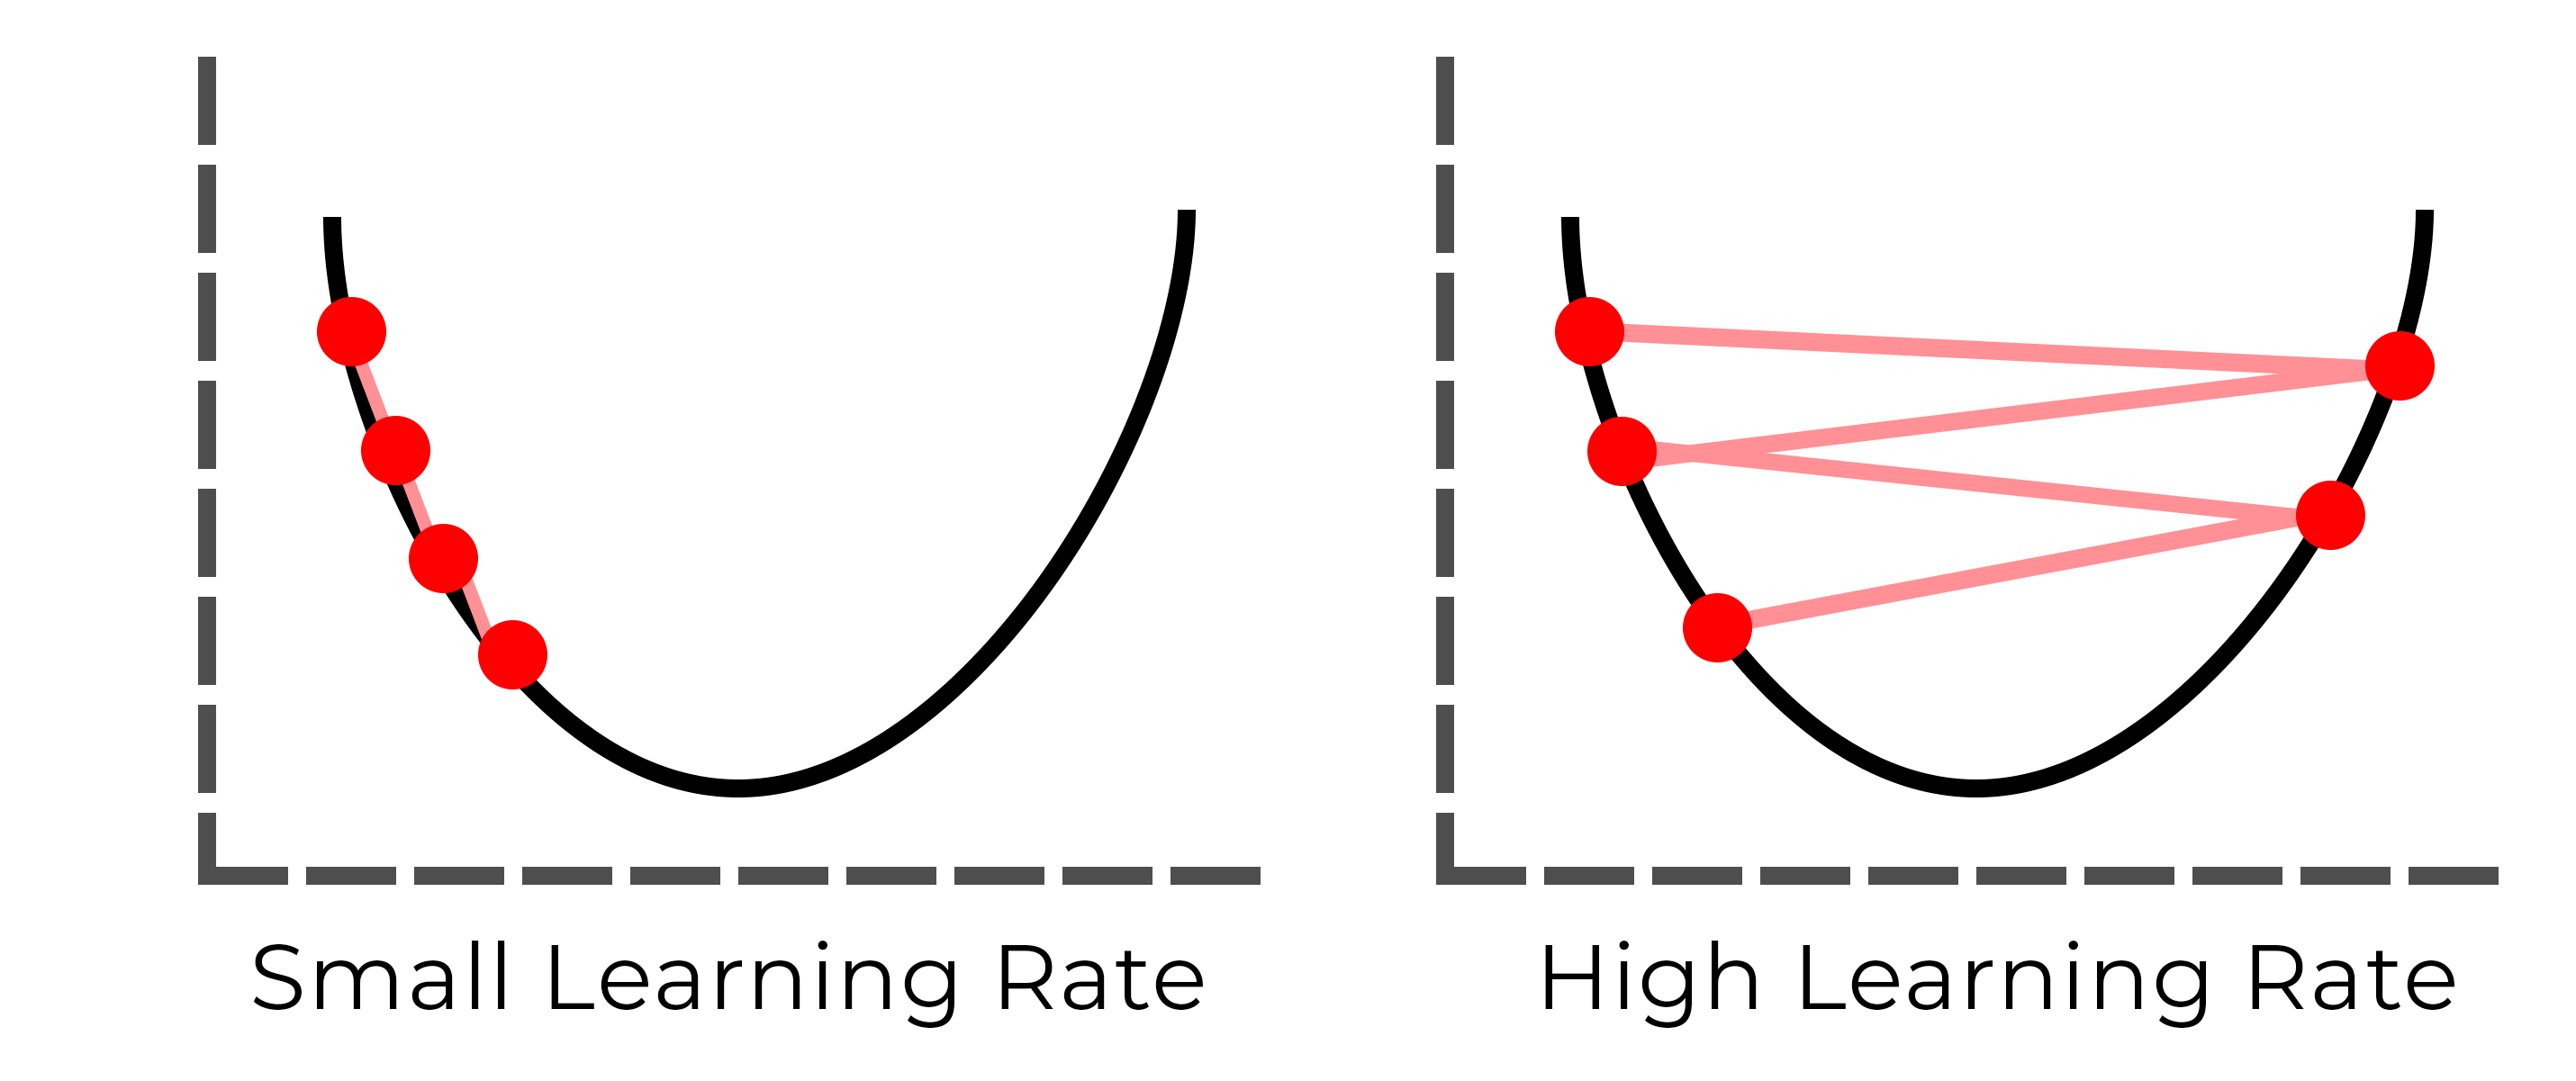
\includegraphics[width=0.7\linewidth]{src/Learning_Rate.png}
  \end{center}
  % NO ES UNA CIENCIA EXACTA
\end{frame}

\begin{frame}{Batch Size}
  \structure{\bf Número de ejemplos de entrenamiento} que se proporcionan a la red antes de que el optimizador actualice los pesos.

  \vspace*{0.8em}

  Un buen tamaño de lote es generalmente \textbf{32}. 
  
  
  Otros válidos son: 32, 64, 128, 256...

  \begin{center}
    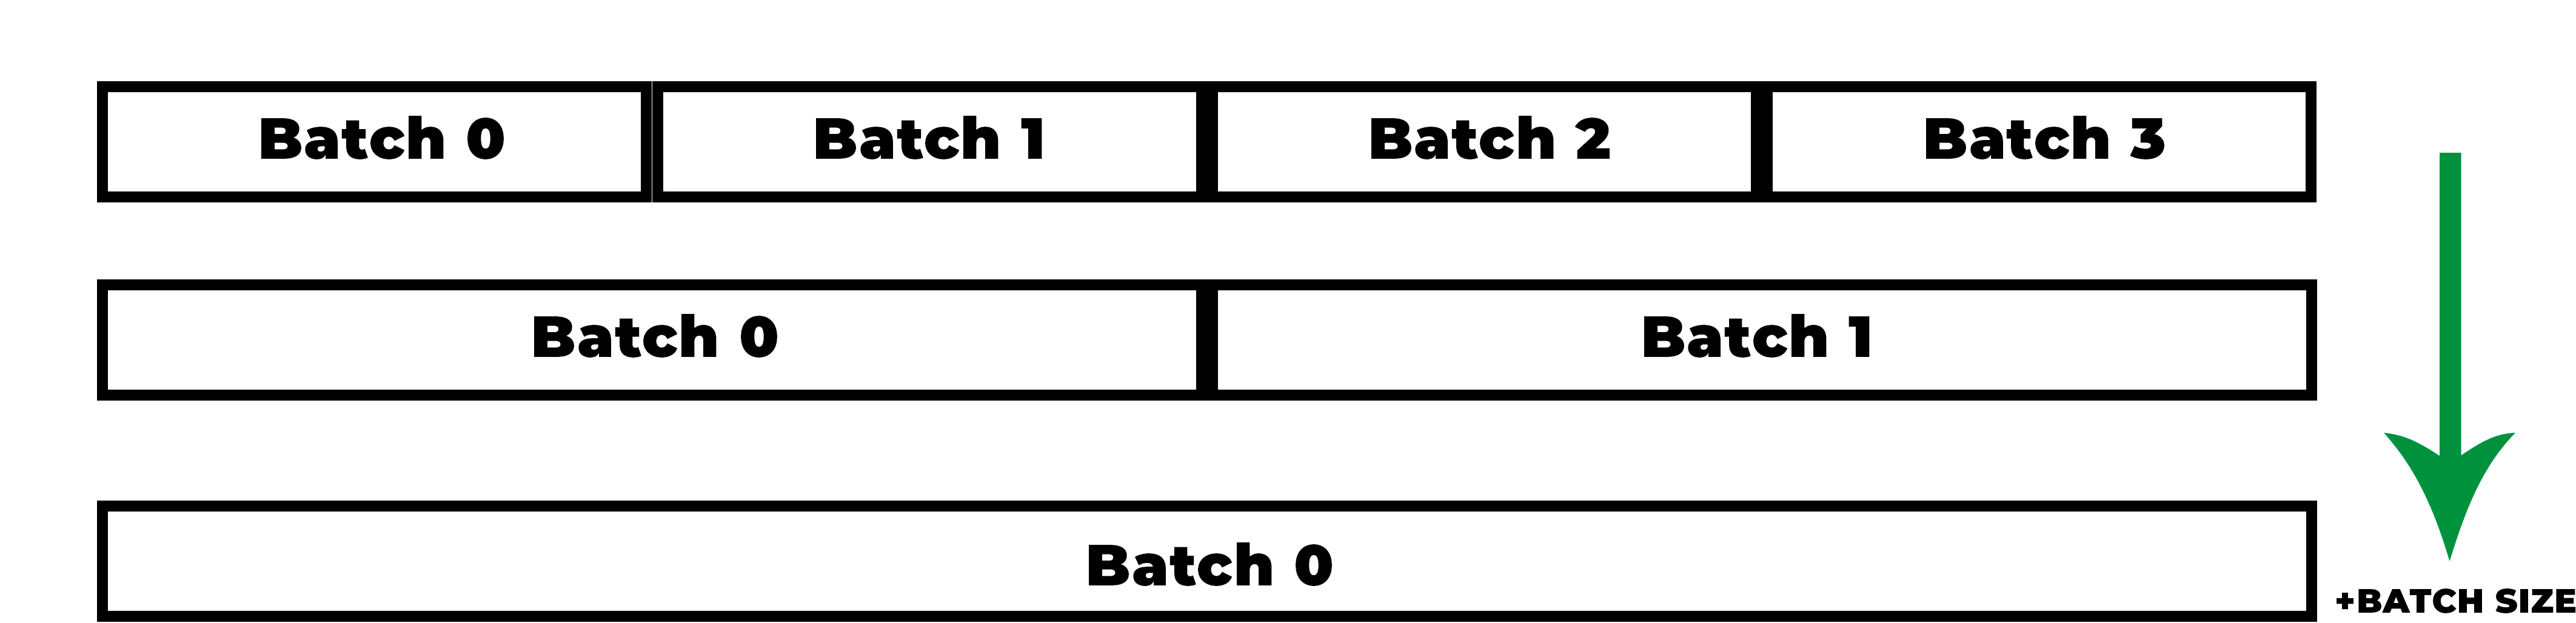
\includegraphics[width=0.9\linewidth]{src/Batch_size.png}
  \end{center}

\end{frame}

\begin{frame}{Numeros de epochs}
  Es el \structure{\bf número de veces que se entrena la red} con el conjunto de datos de entrenamiento.

  \begin{center}
    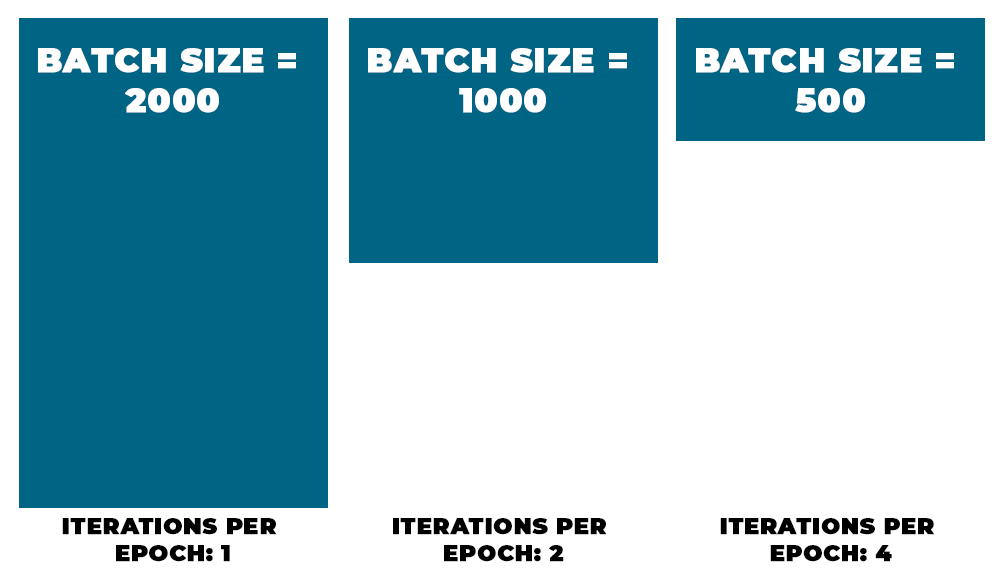
\includegraphics[width=1\linewidth]{src/Iterations-Epoch.png}
  \end{center}

\end {frame}

\begin{frame}{En resumen}
  Mientras que \textbf{$EPOCH < n\_epoch$}
  
  
  \hspace{0.8em}Tomamos una porción de datos \textbf{$\#BATCH\_SIZE$} y la pasamos por la 
  

  \hspace{0.8em}red, calculamos la perdida \textbf{(función de perdida)} y actualizamos los 
  
  
  \hspace*{0.8em}pesos \textbf{(optimizadores).}
  
  
  Fin Mientras

  \begin{center}
    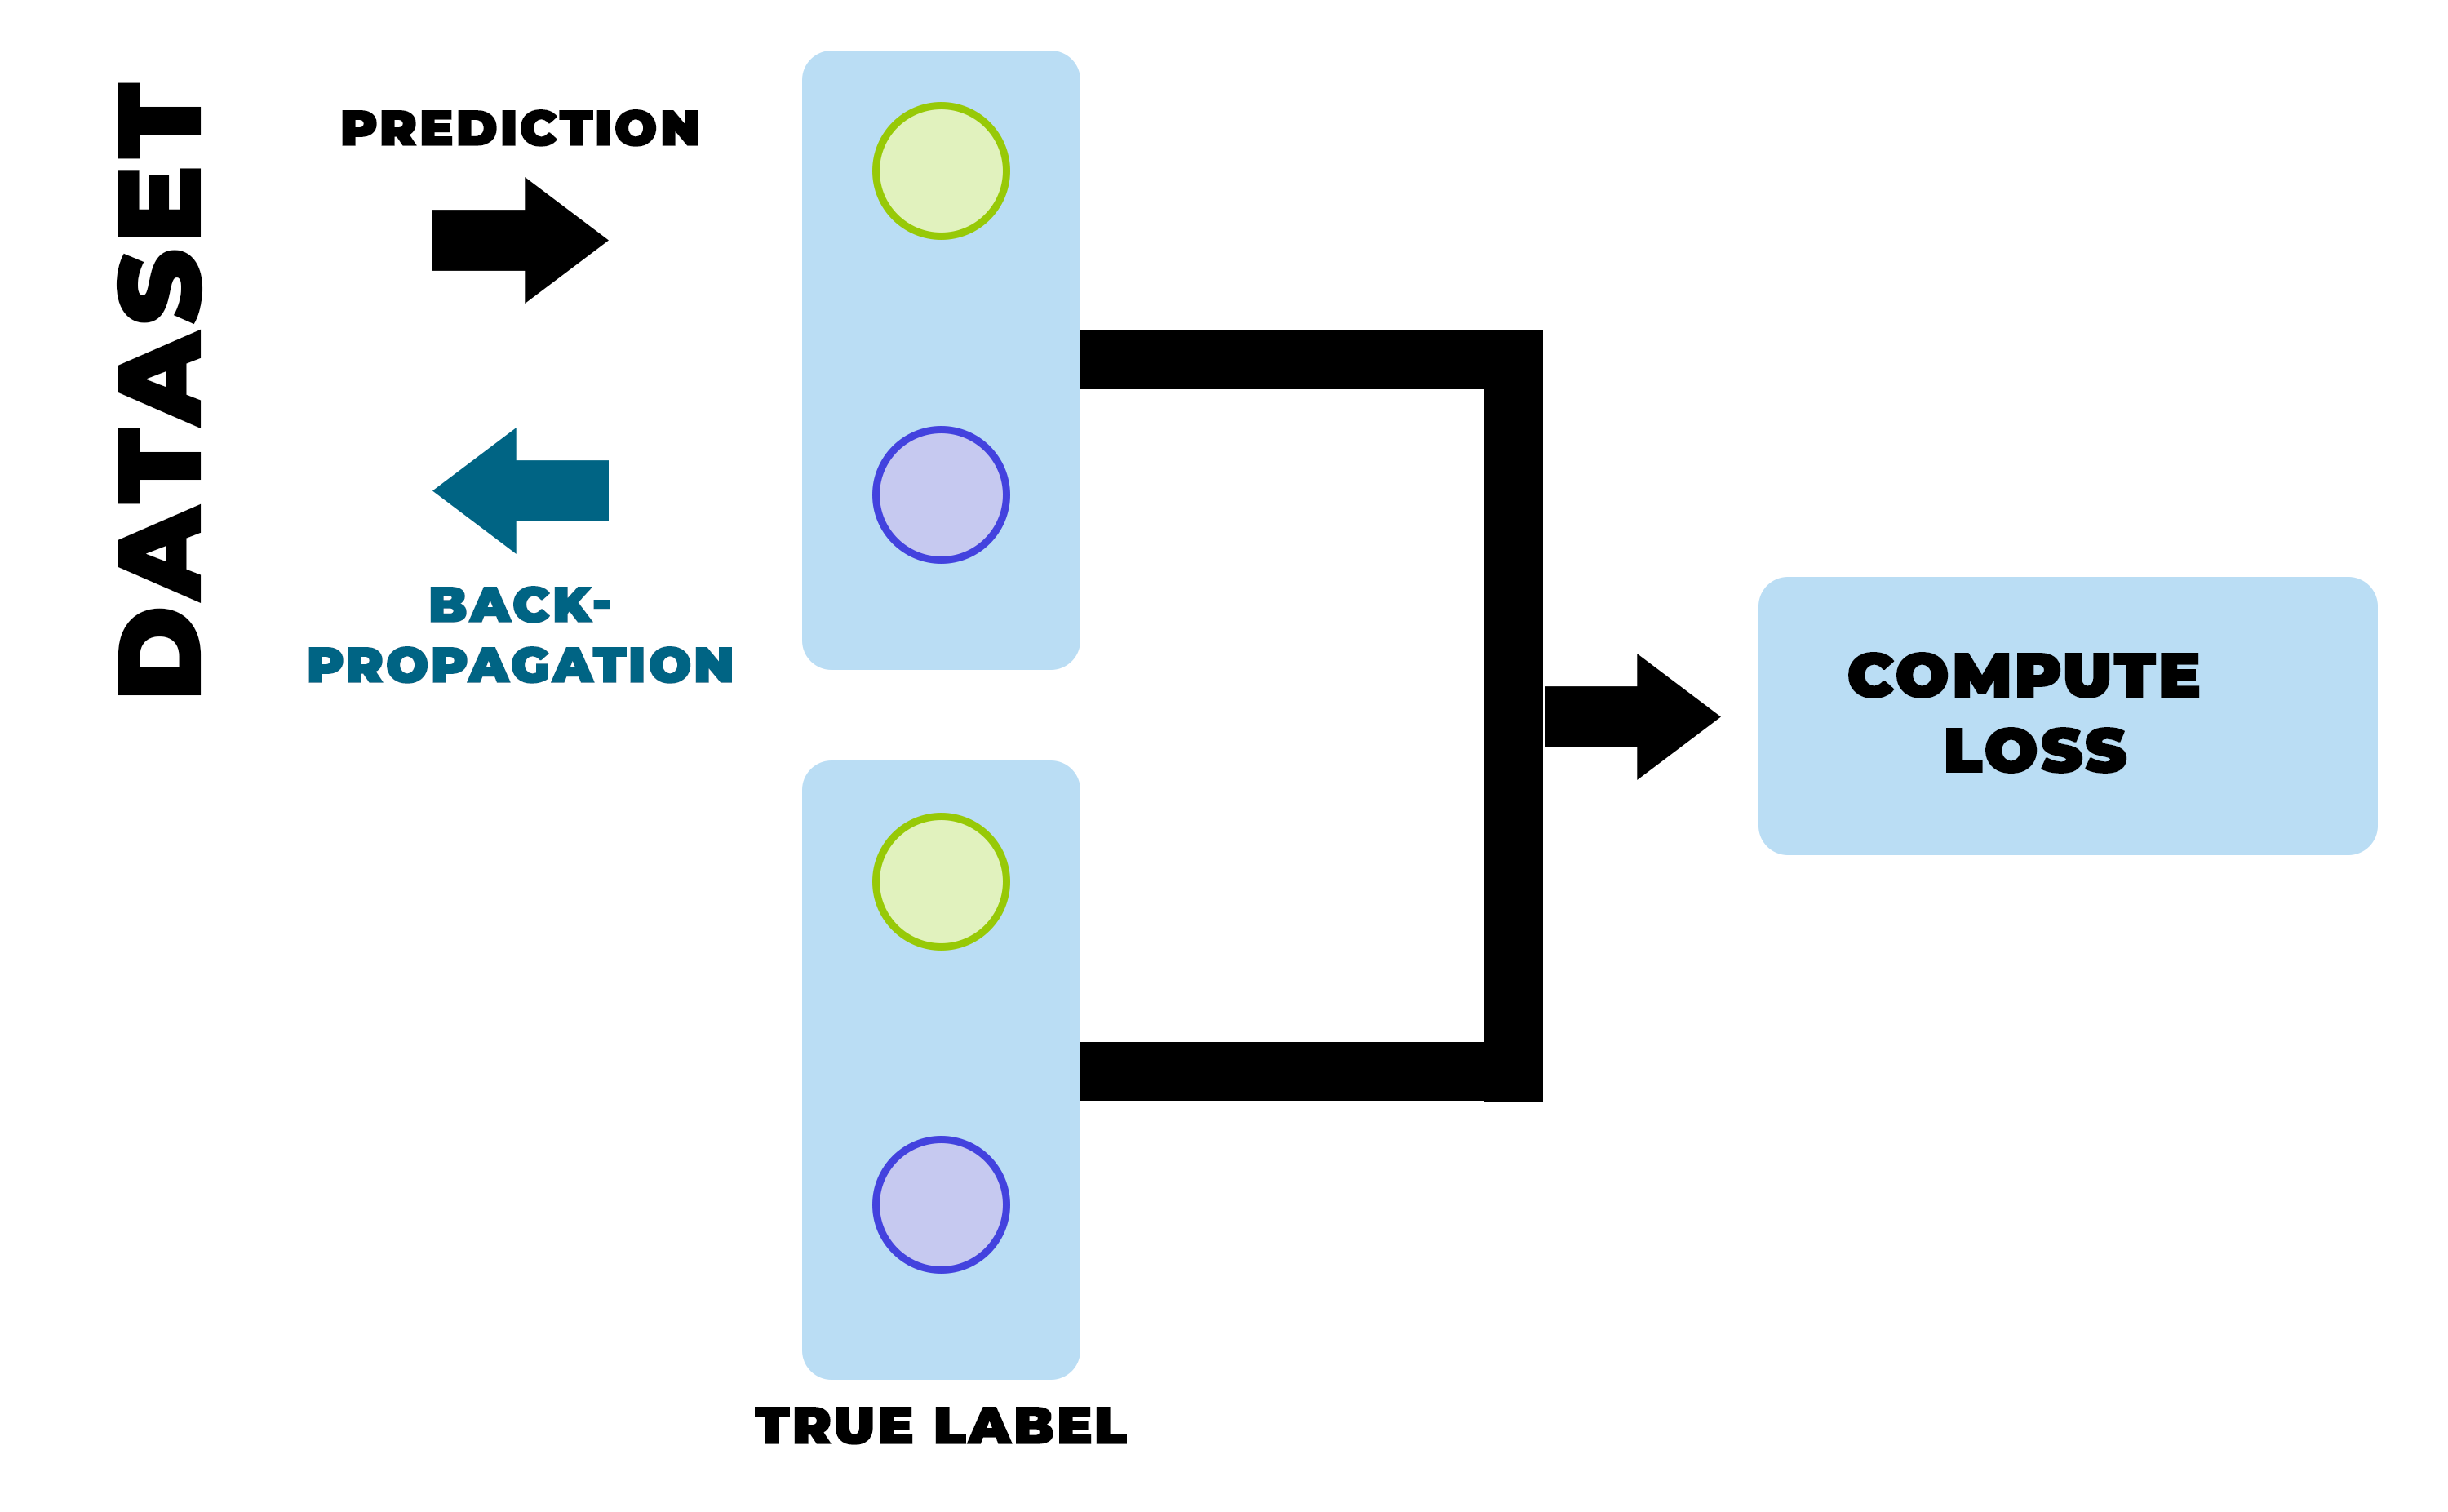
\includegraphics[width=0.7\linewidth]{src/Resumen.png}
  \end{center}
  
  
  
  %Mostrar ejemplo de entrenamiento en tensorflow
\end{frame}

\begin{frame}{Frameworks}
  Principalmente hay dos frameworks que se utilizan:
  \begin{itemize}
    \item \structure{\bf TensorFlow} es una biblioteca de código abierto para aprendizaje automático a través de un rango de tareas, y desarrollado por \textbf{Google} para satisfacer sus necesidades de sistemas capaces de construir y entrenar redes.
    \item \structure{\bf PyTorch} es una biblioteca de aprendizaje automático de código abierto basada en la biblioteca de Torch, utilizado para aplicaciones como visión artificial y procesamiento de lenguajes naturales, principalmente desarrollado por el Laboratorio de Investigación de Inteligencia Artificial de \textbf{Facebook} (FAIR). 
  \end{itemize}
  
  \begin{center}
    
\includegraphics[width=0.7\linewidth]{src/Py-torch-tensorflow.png}
  \end{center}

% Añadir imagenes de tensorflow y pytorch

\end{frame}

\section{Ejemplos prácticos}
\begin{frame}{Ejemplos prácticos}
  La idea de esta sección es ir mostrando una serie de ejemplos prácticos,
  para que se vea como se implementa una red neuronal en la práctica.

  \vspace*{0.8em}

  Para ello tenemos que responder:
  \begin{itemize}
    \item ¿Es una red neuronal adecuada para nuestro problema?
    \item ¿Cuál va a ser nuestros \alert{datos de entrenamiento}?
    \item ¿Cuál es nuestra \alert{arquitectura}?
    \item ¿Qué hiperparámetros escoger?
  \end{itemize}
\end{frame}
% Añadir cuando no es buena idea una red neuronal
\begin{frame}{Conecta4 AI}
\Large{\textbf{Datos de entrenamiento}}

\vspace*{0.8em}

Mediante el \structure{\bf algoritmo Minimax,} se genera una tabla de entrenamiento que recoge para una posición del tablero, la mejor jugada que se puede hacer.
 \begin{table}[ht]
  \centering
  \begin{tabular}{|c|c|c|c|}
  \hline
  Estado Tablero  & Actua  & Mejor acción  \\
  \hline
 $\begin{bmatrix}
  1 & 0 & 0 & 0 & 0 & 0 & 0 \\
  1 & 2 & 0 & 0 & 0 & 0 & 0 \\
  2 & 1 & 0 & 0 & 0 & 0 & 0 \\
  2 & 2 & 0 & 0 & 0 & 0 & 0 \\
  1 & 2 & 0 & 2 & 0 & 1 & 0 \\
  2 & 2 & 1 & 1 & 0 & 1 & 1 \\
 \end{bmatrix}$ & 2 & 4 \\
  \hline
  \end{tabular}
 \end{table}

%\url{https://es.wikipedia.org/wiki/Minimax#/media/Archivo:Minimax.svg}

\end{frame}

\begin{frame}{Arquitectura}
  \alert{\Large{Input (Imagen) $\rightarrow$ Convolución $\rightarrow$ Densa $\rightarrow$ Salida (7)}}
  \begin{center}
    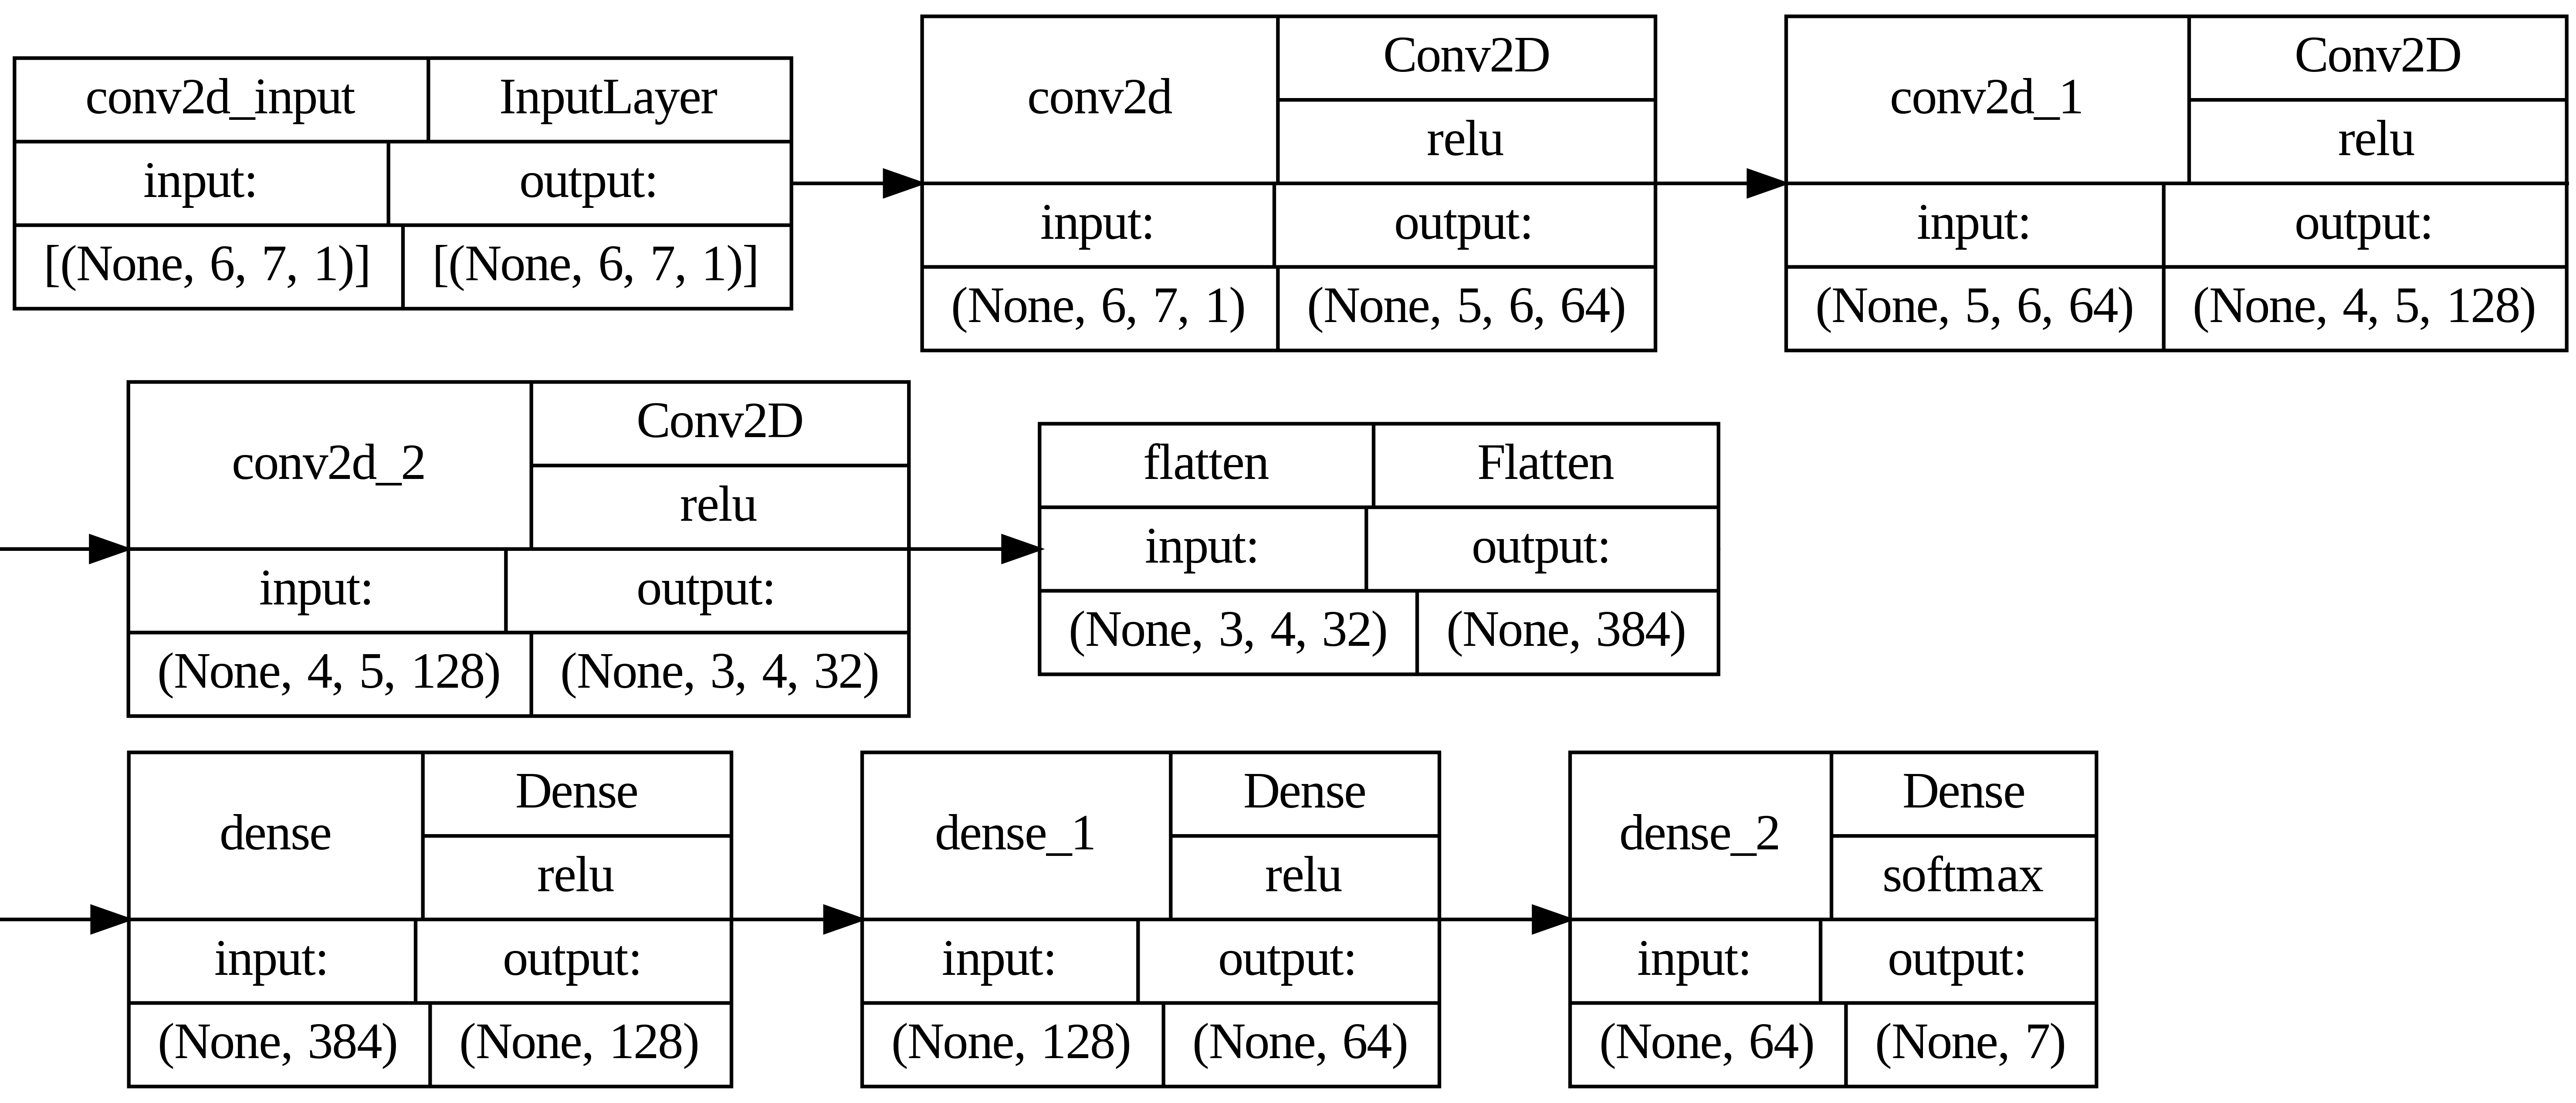
\includegraphics[width=1\linewidth]{src/model (1).png}
  \end{center}
\end{frame}

\begin{frame}{Convolución}
% https://towardsdatascience.com/conv2d-to-finally-understand-what-happens-in-the-forward-pass-1bbaafb0b148
Son muy importantes cuando tenemos que procesar imágenes, puesto
que ayudan a \alert{simplificar la imagen,} para luego pasarlo por una capa densa y obtener un buen resultado.
\begin{center}
  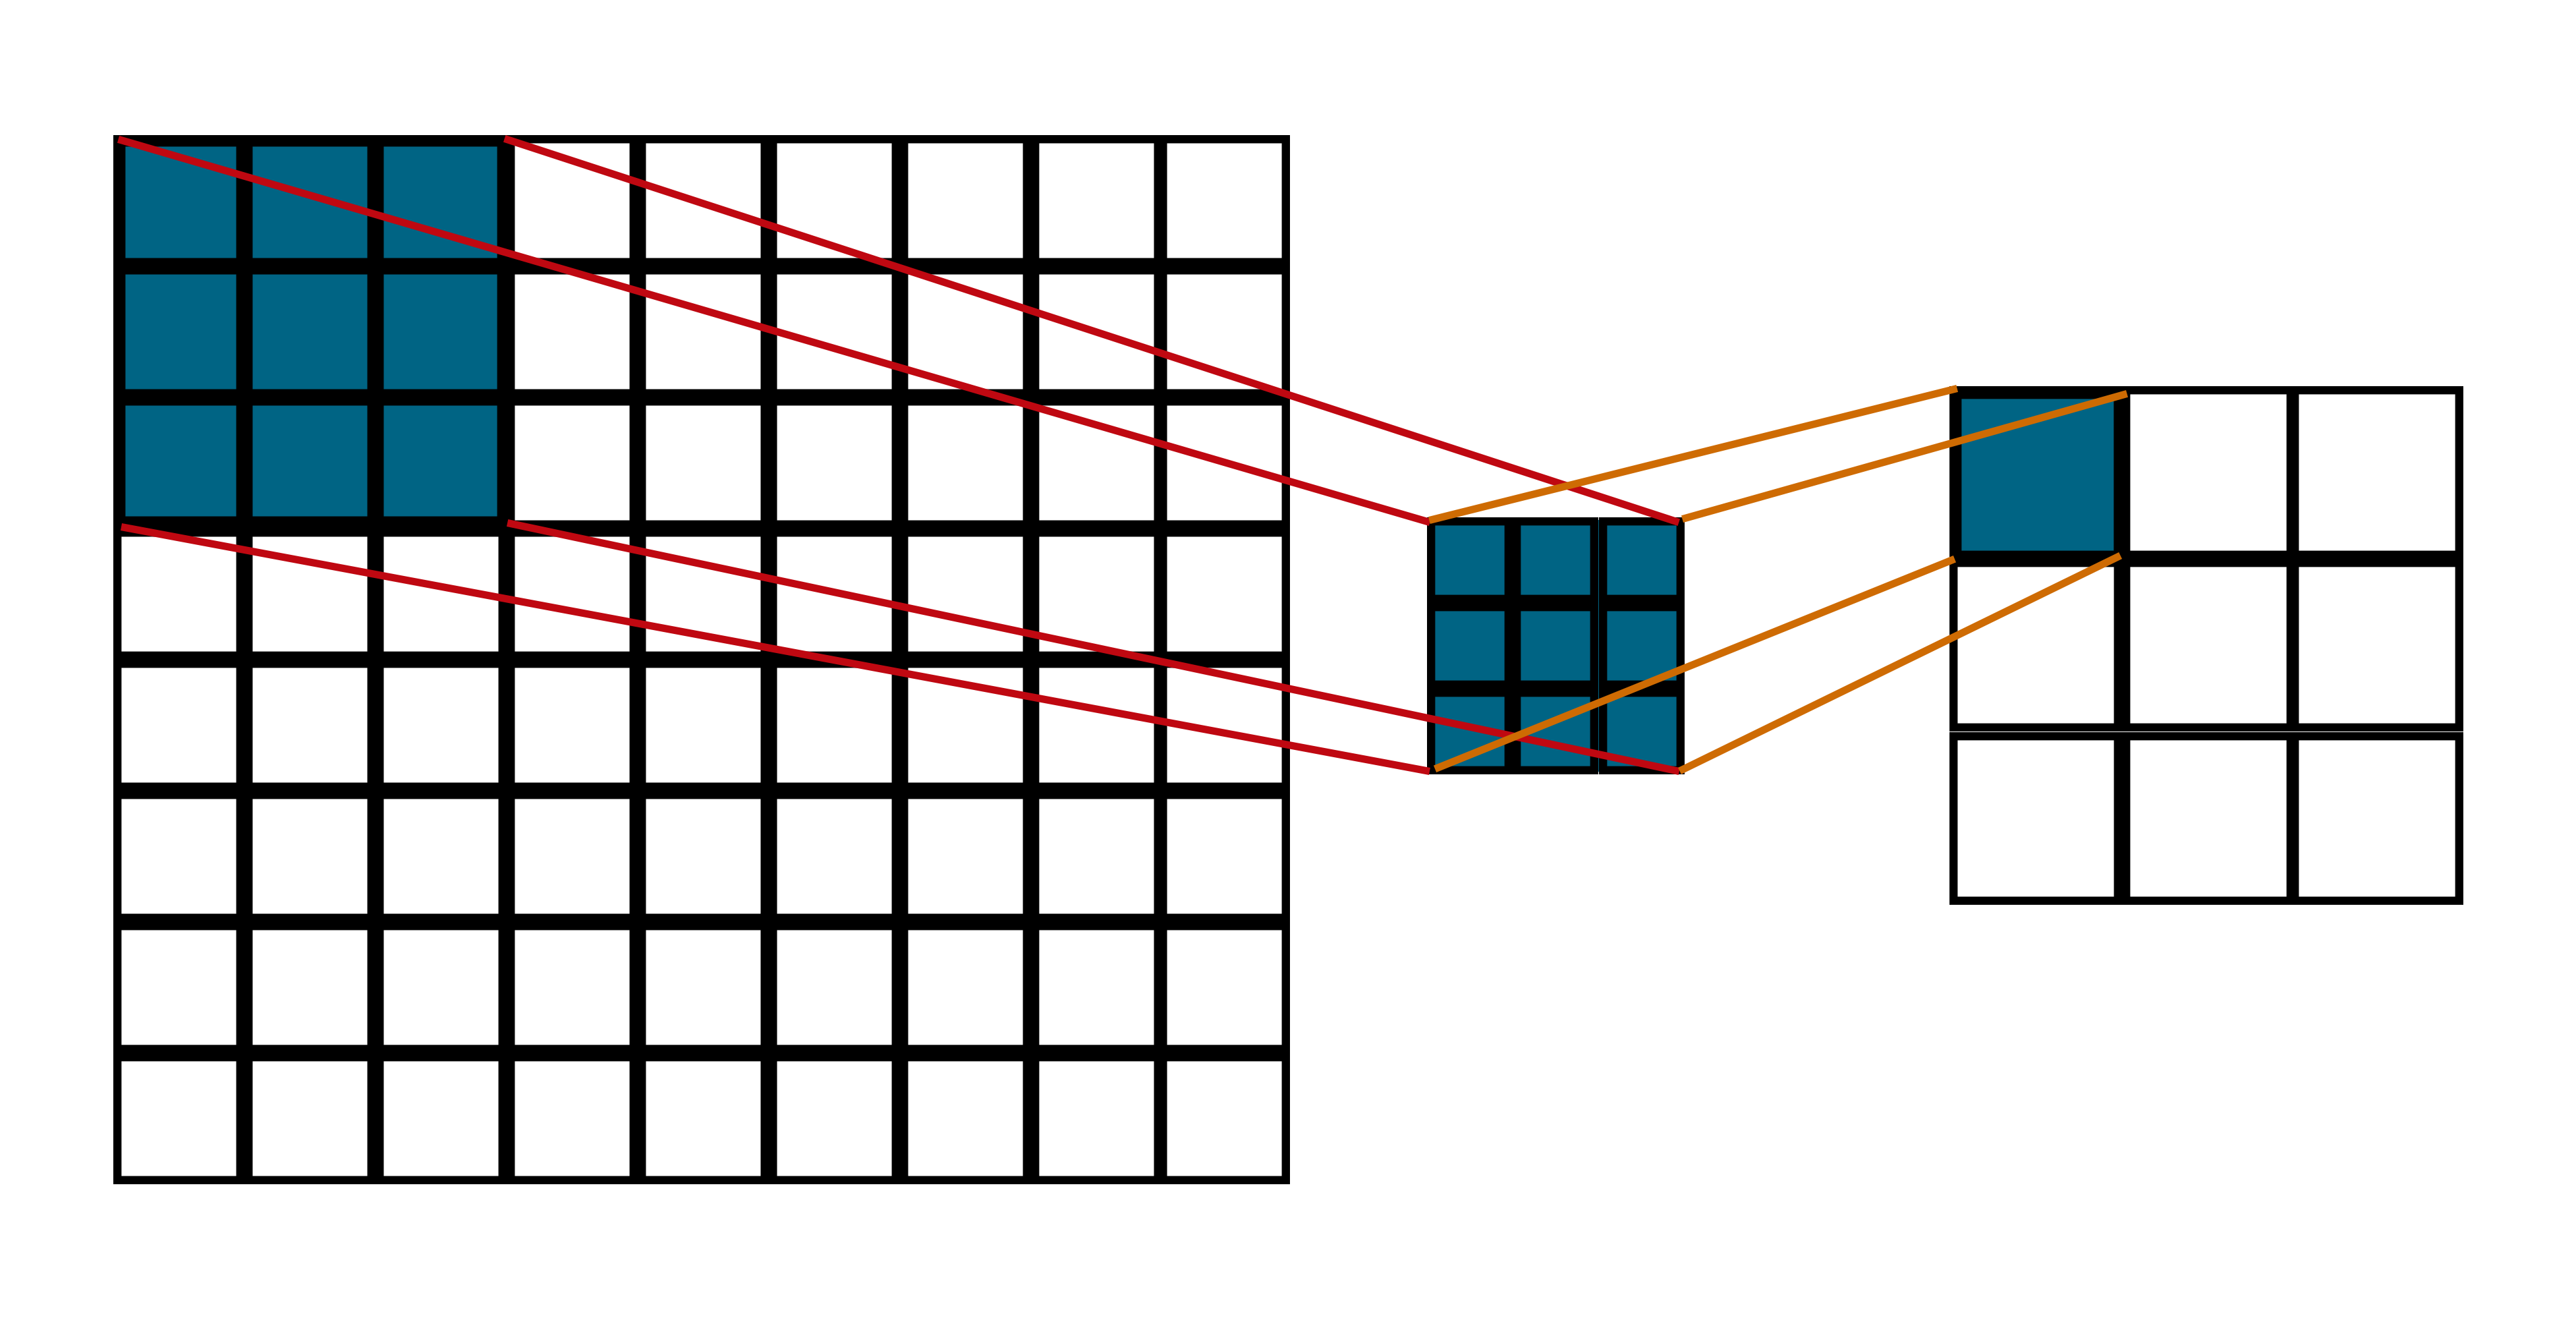
\includegraphics[width=1\linewidth]{src/Conv2D.png}
\end{center}
\end{frame}

\begin{frame}{Hiperparámetros}
  $$train\_size = 90000$$
  $$val\_size = 5000$$
  $$test\_size = 5000$$
  
  
  $$BATCH\_SIZE = 64$$
  $$EPOCHS = 512$$
  $$LR = 0.001$$
  
  \textbf{¿Función de perdida?}

  
  \alert{Clasificación} o \alert{Regresión}


  $LOSS = 'sparse\_categorical\_crossentropy'$
\end{frame}

\begin{frame}{Criptografia AI}
  \Large{\textbf{Datos de entrenamiento}}

  \vspace*{0.8em}

  \begin{itemize}
    \item Imagenes aleatorias de tamaño 256x256
    \item Texto aleatorio en formato ASCII
      \textbf{$$[ 30, 250, 240,100, 30, 40, 60]$$}
  \end{itemize}
  \begin{center}
    
\includegraphics[width=0.45\linewidth]{src/example_input.png}
  \end{center}

\end{frame}

\begin{frame}{Arquitectura}
  \textbf{AutoEncoder}

  \vspace*{0.8em}

  \begin{itemize}
    \item \textbf{\alert{Encoder:}} Incrusta el texto en la imagen devolviendo una imagen modificada.
    \item \textbf{\alert{Decoder:}} Devuelve el texto incrustado en la imagen.
  \end{itemize}

\begin{center}
  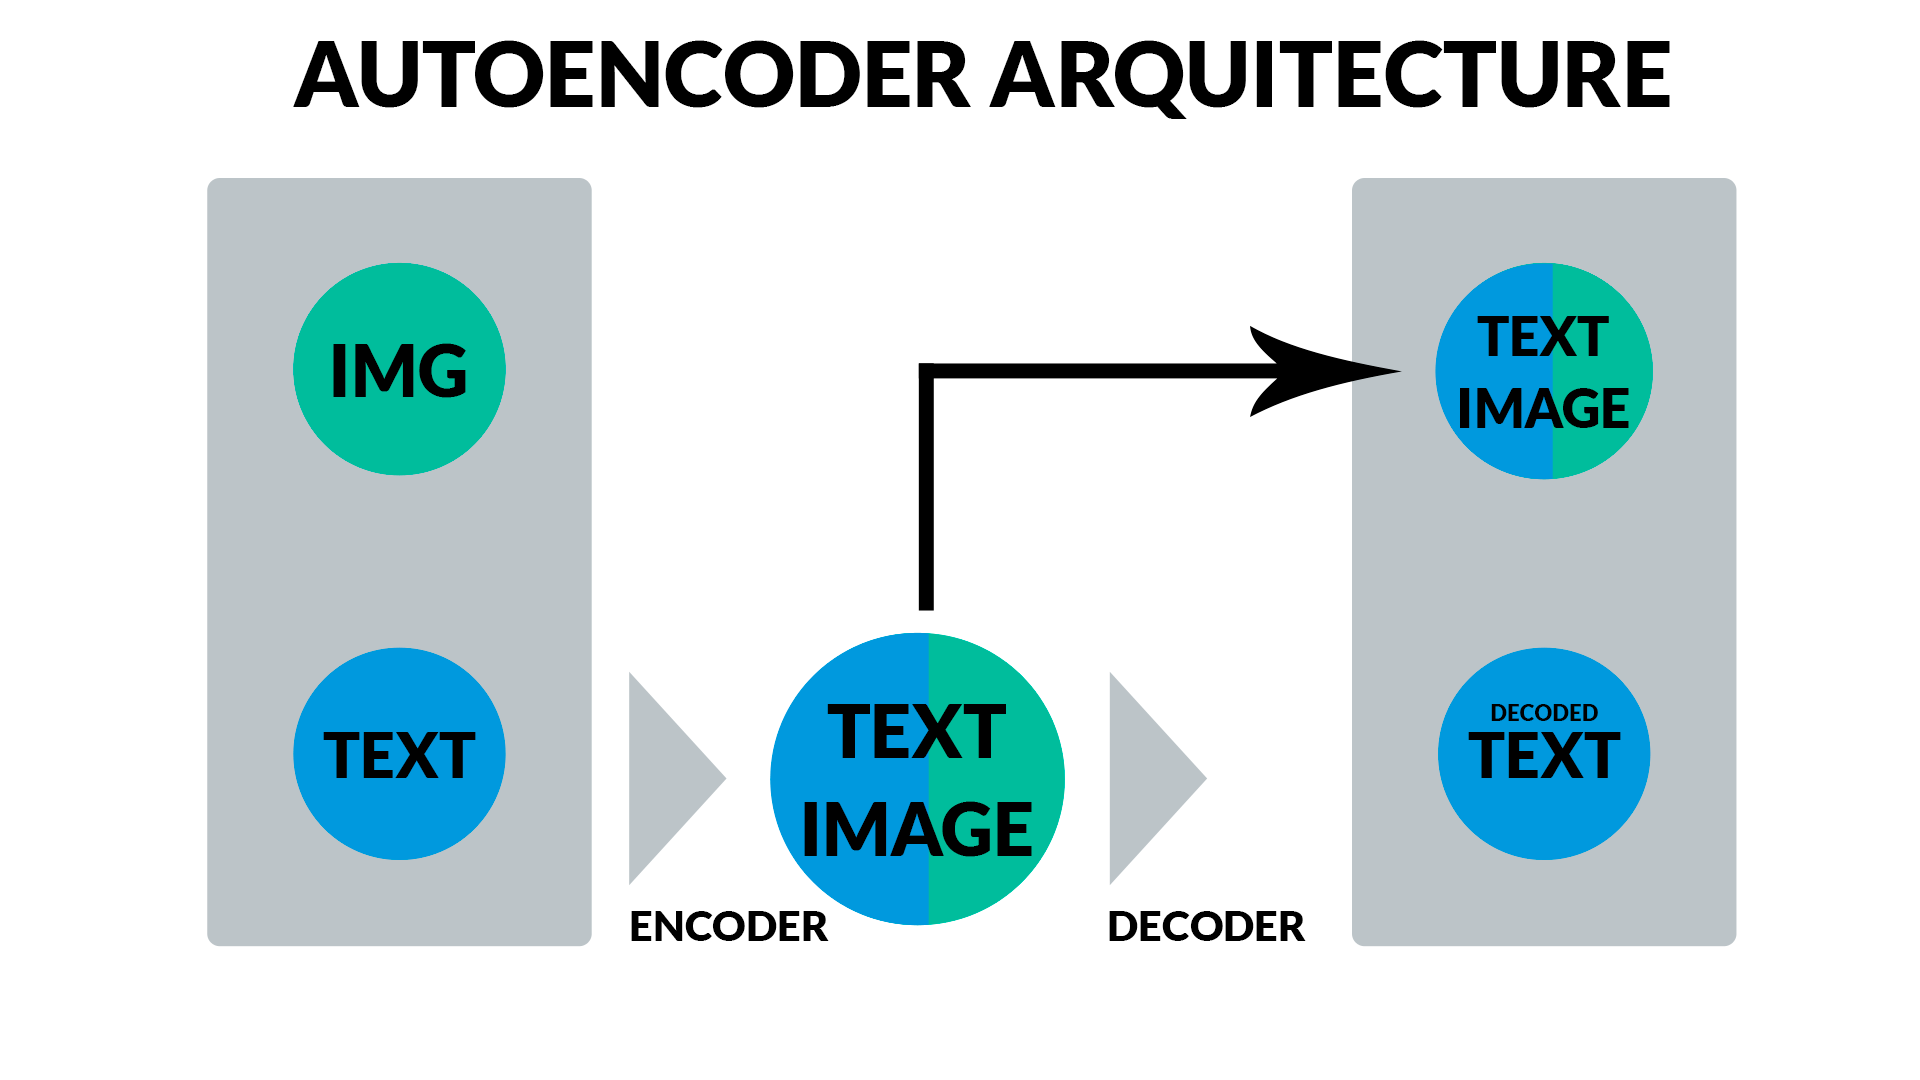
\includegraphics[width=0.75\linewidth]{src/AutoEncoder-arq.png}
\end{center}

\end{frame}

\begin{frame}{Encoder}
  % Añadir imagen de encoder y decoder
  \begin{center}
    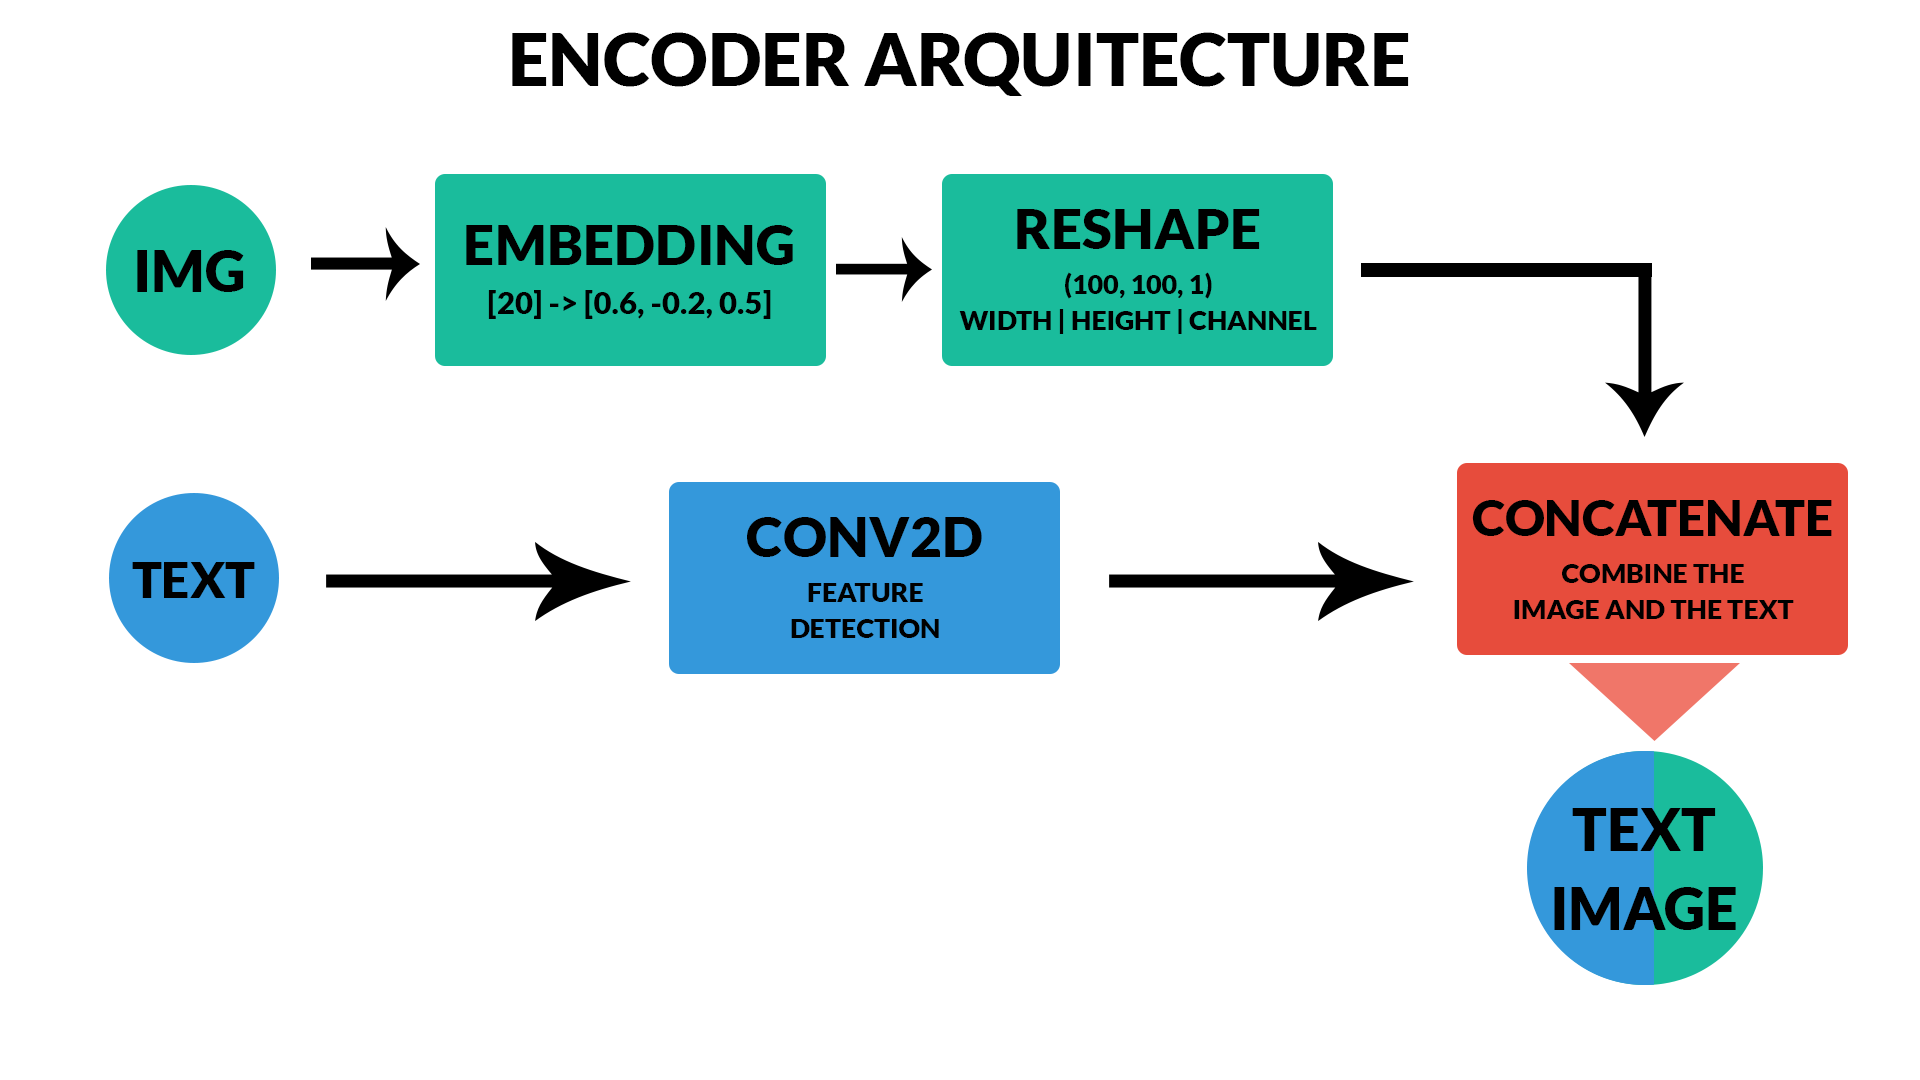
\includegraphics[width=1\linewidth]{src/Encoder-arq.png}
  \end{center}
\end{frame}

\begin{frame}{Decoder}
  \begin{center}
    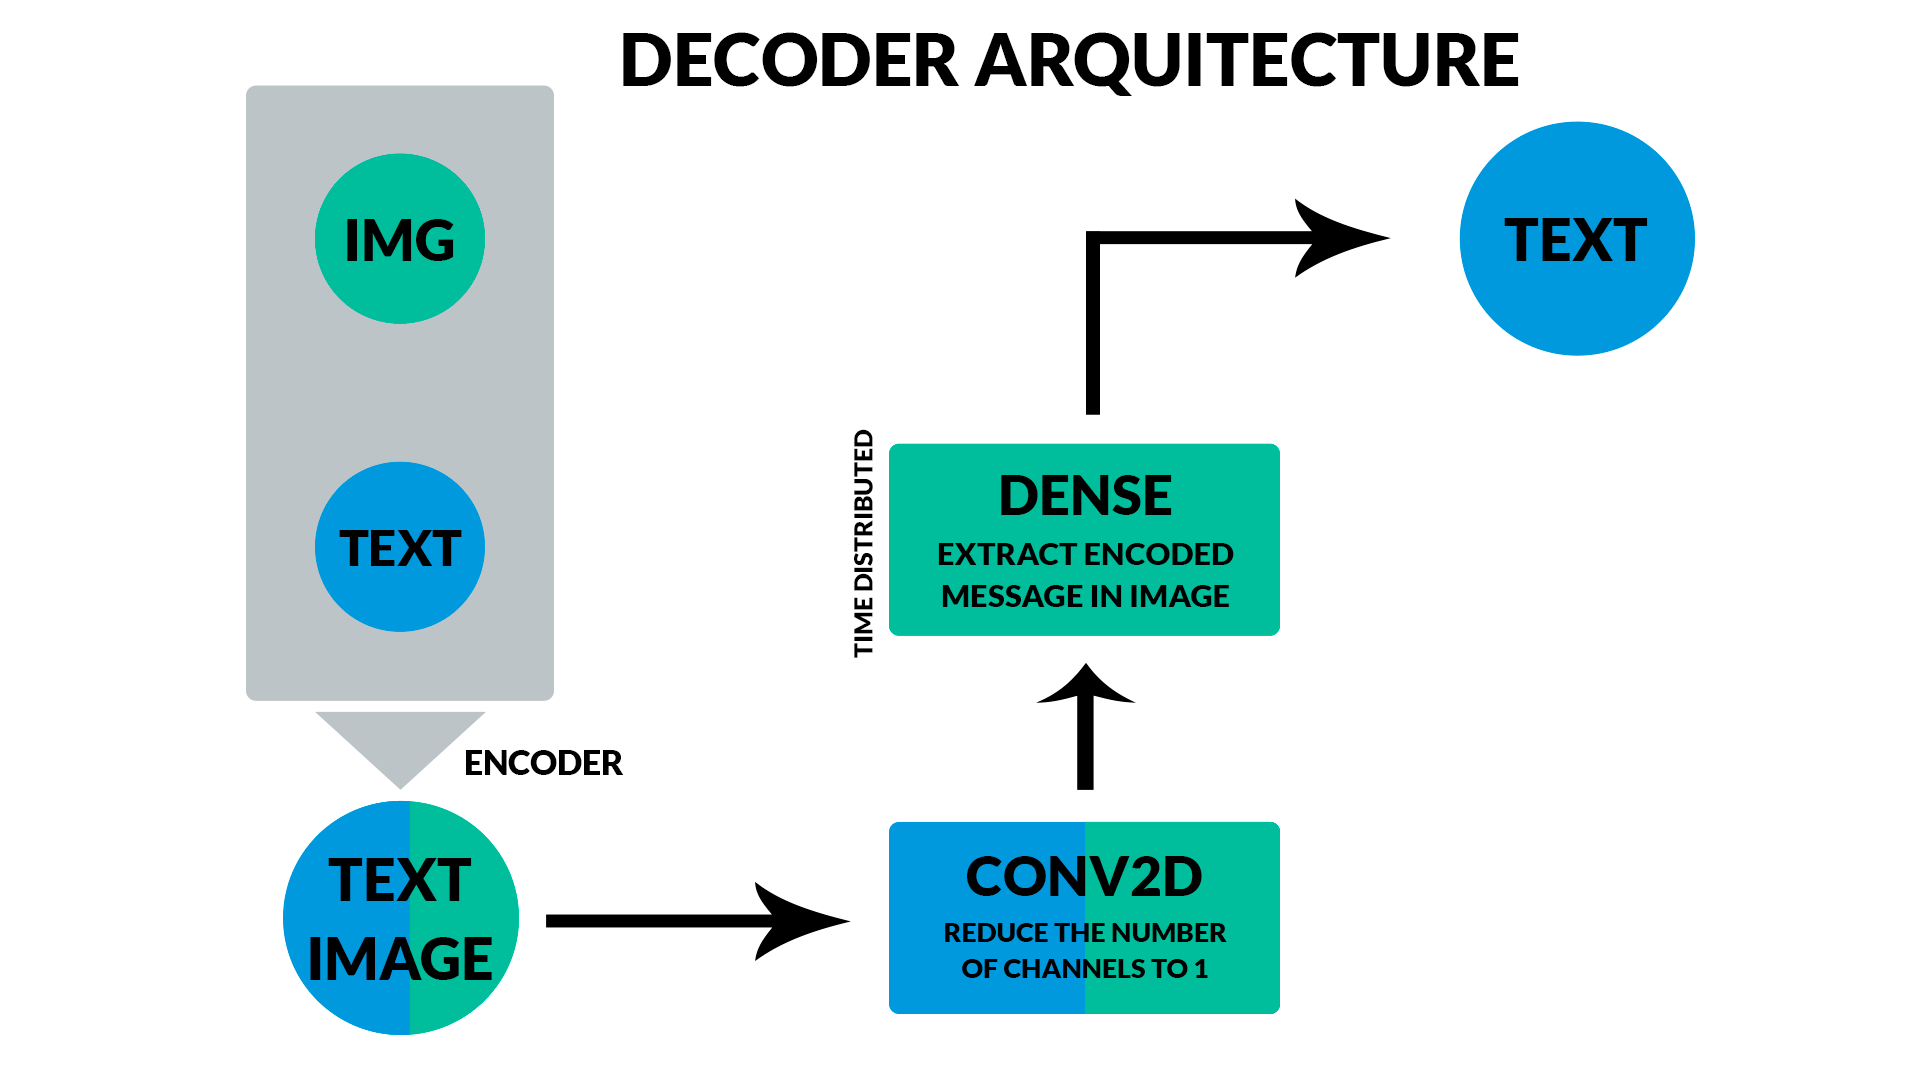
\includegraphics[width=1\linewidth]{src/Decoder-arq.png}
  \end{center}
\end{frame}



\begin{frame}{Hiperparámetros}

  $$epochs=512$$ 
  $$steps\_per\_epoch=512$$
  $$BATCH\_SIZE = 64$$
  $$LR = 0.001$$

  \vspace*{0.8em}

  \textbf{Funciones de perdida}
  \begin{itemize}
    \item \alert{$1-$ MSE}
    \item \alert{$2-$ Categorical Cross Entropy}
  \end{itemize}

\end{frame}

\begin{frame}{Doodle}
  \textbf{Datos de entrenamiento}

  \vspace*{0.8em}
\begin{itemize}
  \item Imagenes \textbf{(Doodles)\footnote{\url{https://quickdraw.withgoogle.com/}}}
  \begin{center}
    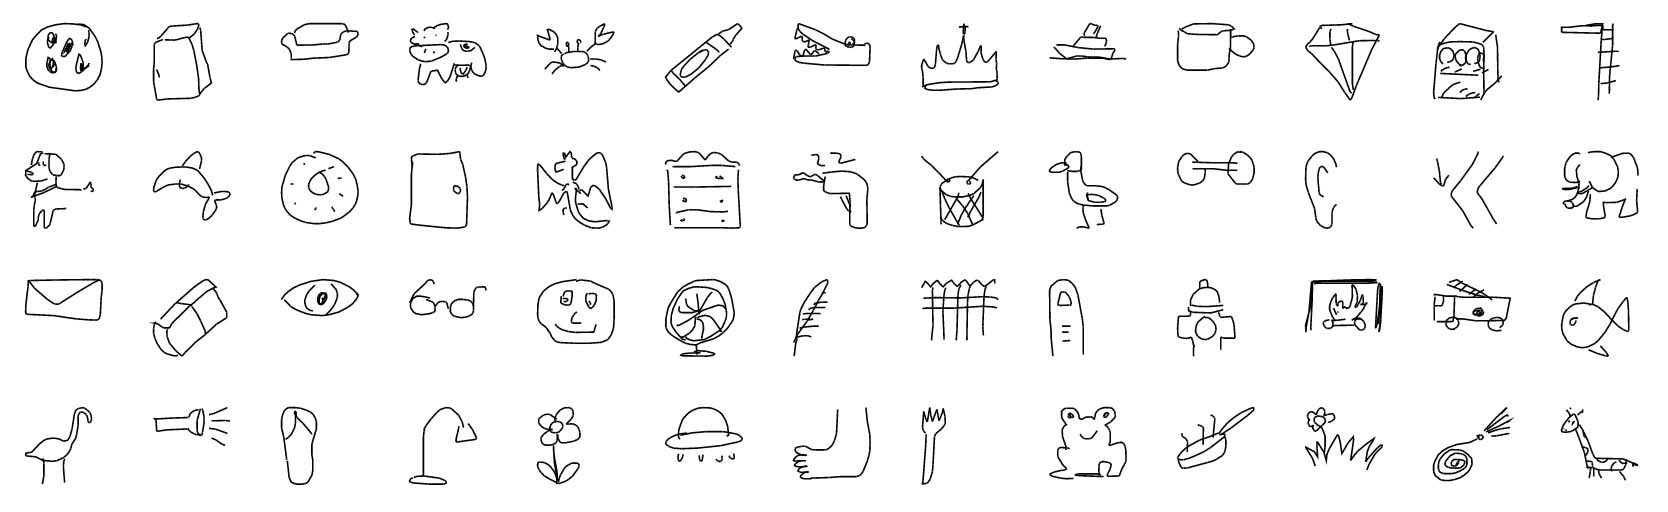
\includegraphics[width=1\linewidth]{src/preview.jpg}
  \end{center}
  \item Categorias:
  $$[aircraft carrier,
  airplane,
  alarm clock,
  ambulance,
  angel...]$$
\end{itemize}
\end{frame}

\begin{frame}{ED}
\Large{
Vamos a resolver la siguiente PDE:
\begin{equation*}
  \begin{cases}
    $$\phi_t + u\phi_x=0, (x,t)\in(0,1)\times(0,1) \\
    \phi(t,0)=\phi(t,1), t\in(0,1) \\
    \phi(0,x)=sin(2\pi x /L), x\in(0,1)$$
  \end{cases}
\end{equation*}

Donde \textbf{$u=1$} es la velocidad y \textbf{$L=1$}, son valores 


escalares constantes.

\vspace*{0.8em}

\structure{\bf Objetivo: $f_{NN} \approx \phi$}
}
\end{frame}

\begin{frame}
  \large{\textbf{Datos de Entrenamiento}}
  \begin{itemize}
    \item \alert{$X_0 = [t_0, \{0,1\}]$} Cantidad: 500
    
    \vspace*{0.5em}

    Proviene de: $\phi(t,0)=\phi(t,1), t\in(0,1)$ 
    \item  \alert{$X_b = [0, x_b]$} Cantidad: 500
    
    \vspace*{0.5em}

    Proviene de: $\phi(0,x)=sin(2\pi x /L), x\in(0,1)$ 

    \item \alert{$X_r=[t_r, x_r]$} Cantidad: 10000
    
    \vspace*{0.5em}
    
    Son puntos aleatorios en $(0,1)\times(0,1)$

  \end{itemize}
\end{frame}

\begin{frame}{Arquitectura}

  \begin{center}
    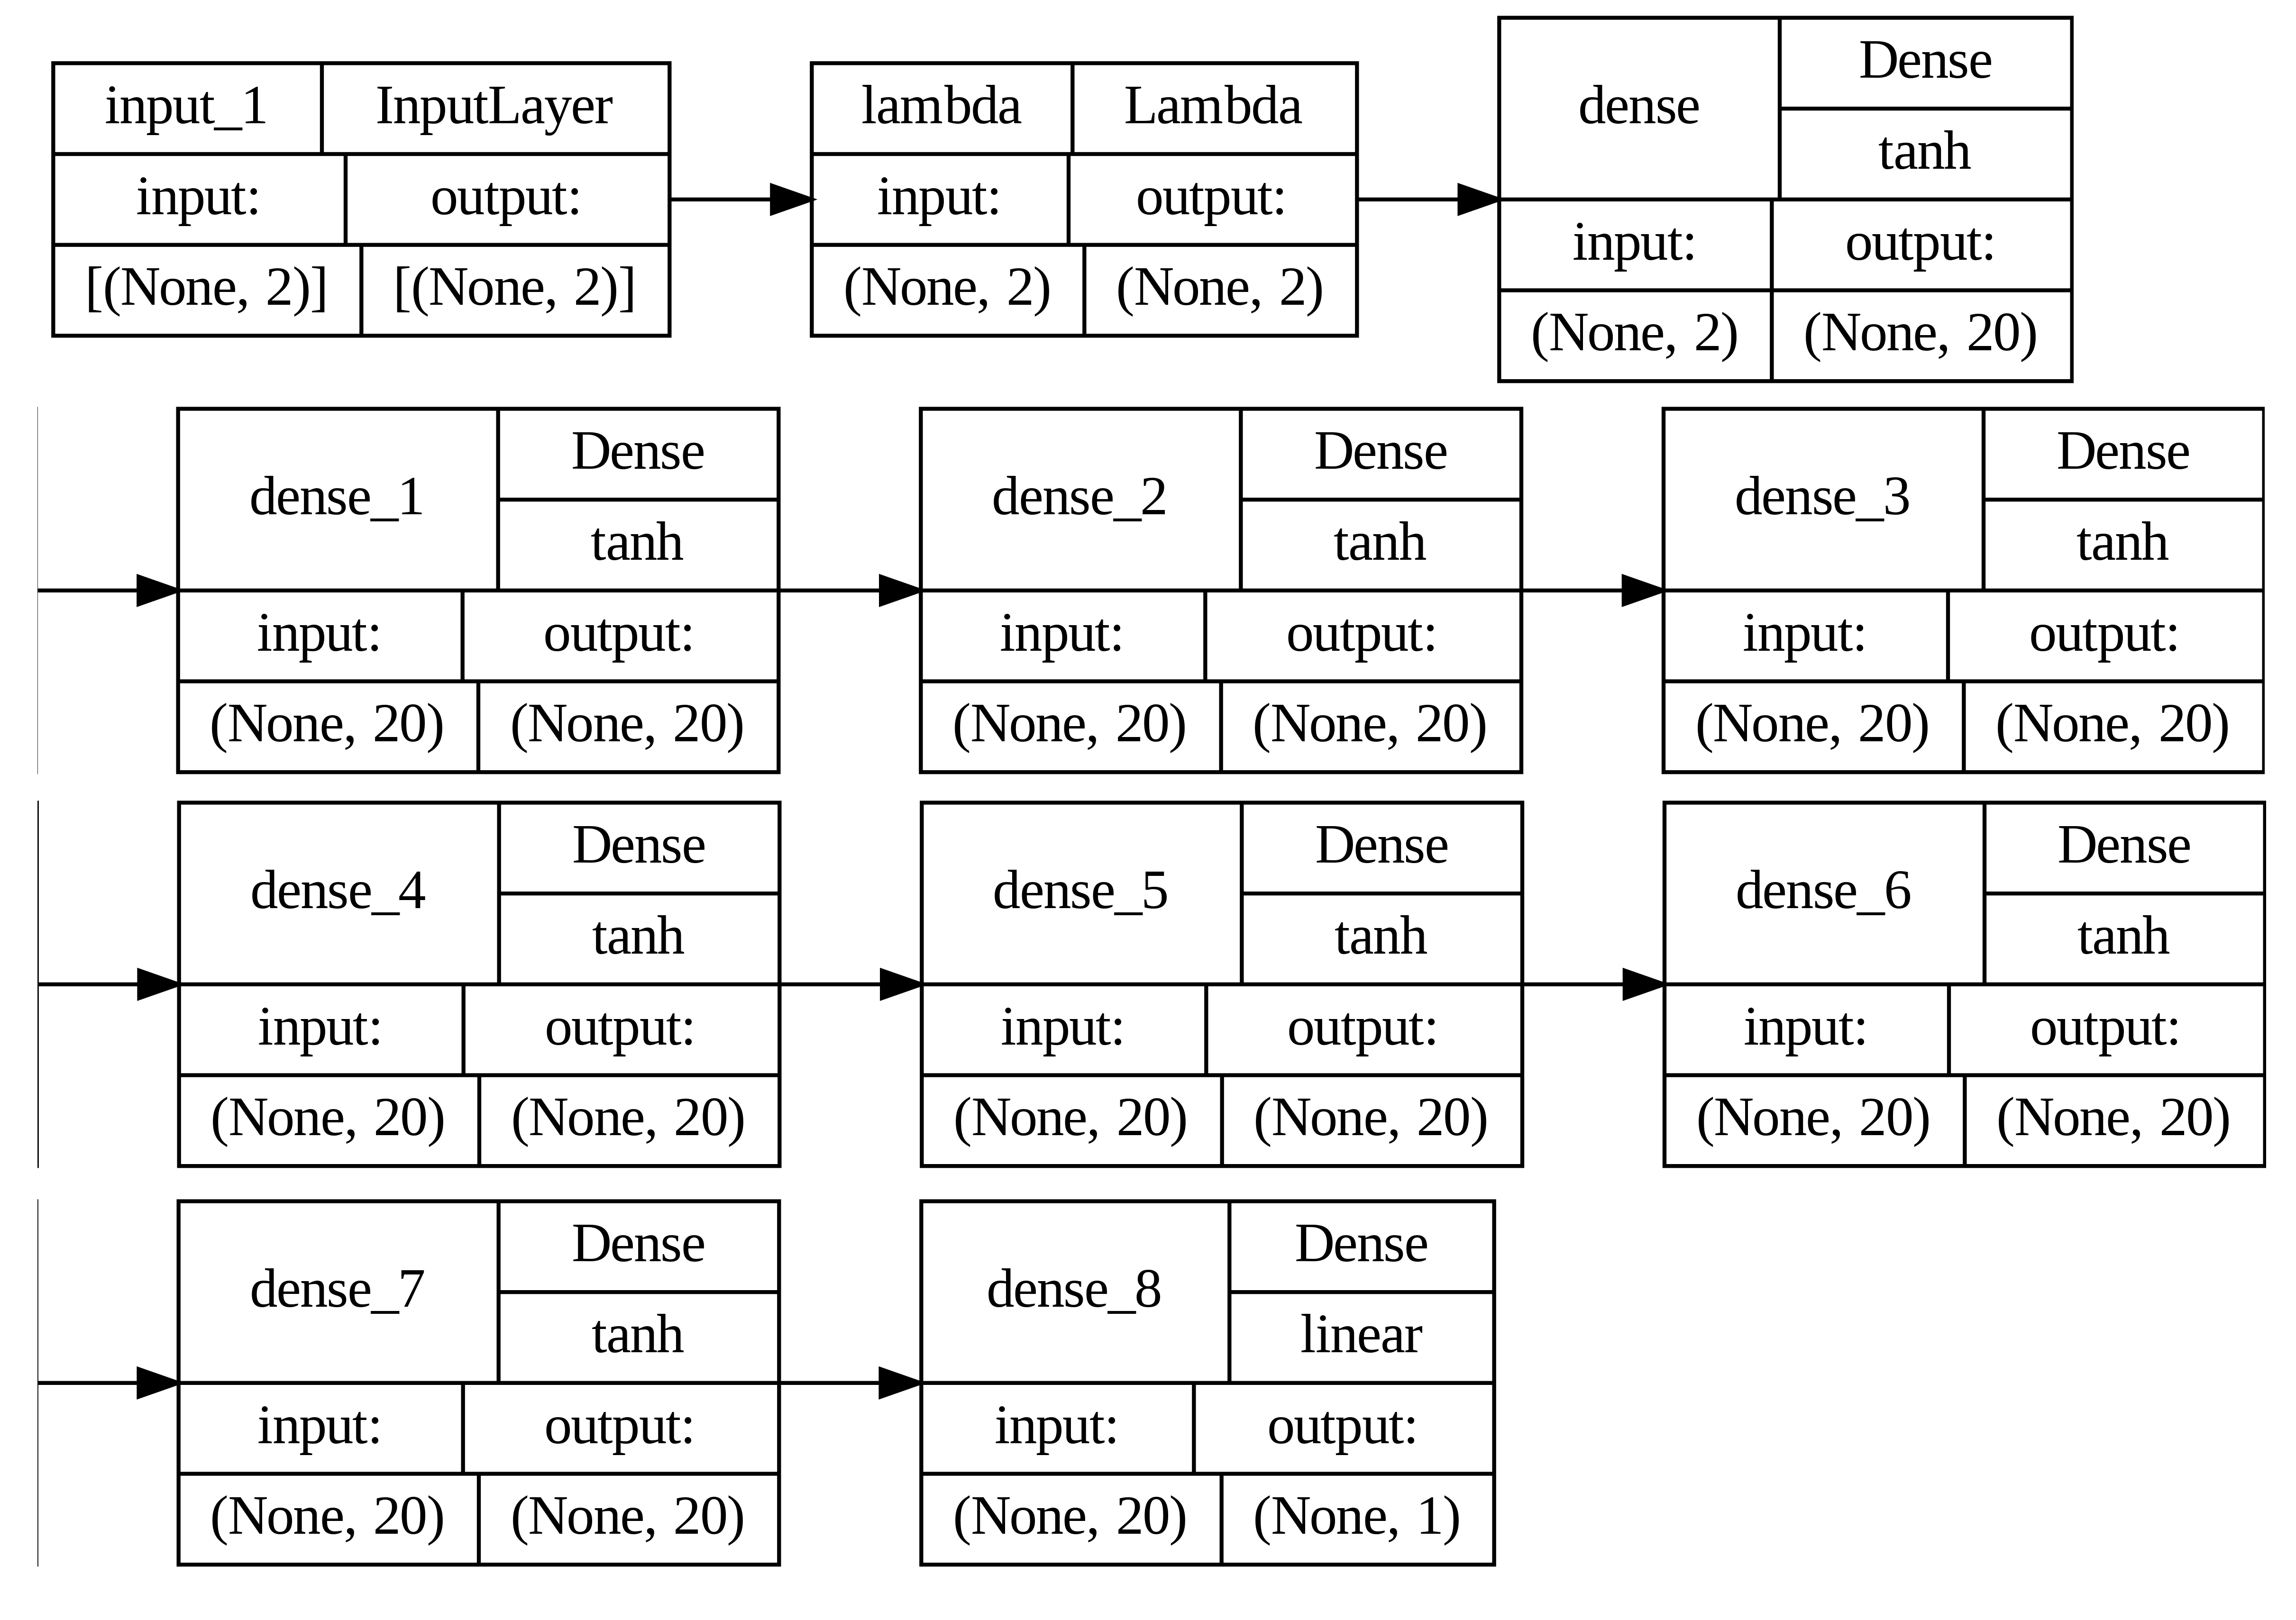
\includegraphics[width=0.8\linewidth]{src/model_ed.png}
  \end{center}
\end{frame}

\begin{frame}{¿Cómo calculamos la pérdida?}

  \begin{itemize}
    
    \item \textbf{Primera Pérdida}

    \vspace*{0.4em}

    Pasamos $X_r = [t_r, x_r]$ por la red neuronal y obtenemos $f_{NN}(t_r, x_r)$
    Aplicando diferenciación automática obtenemos $\frac{\partial f_{NN}}{\partial t}$ y $\frac{\partial f_{NN}}{\partial x}$
    \alert{$$LOSS += \left (\frac{\partial f_{NN}}{\partial t} + u\frac{\partial f_{NN}}{\partial x}\right )^2$$}
    
    \item \textbf{Segunda Pérdida}
    
    \vspace*{0.4em}
    
    Pasamos $X_b = [t_b, \{0,1\}]$ por la red neuronal y obtenemos $f_{NN}(t_b, x_b)$
    \alert{$$LOSS += (f_{NN}(t_b,0) - f_{NN}(t_b,1))^2$$}

    \item \textbf{Tercera Pérdida}
    
    \vspace*{0.4em}
    
    
    Pasamos $X_0 = [0, x_0]$ por la red neuronal y obtenemos $f_{NN}(t_0, x_0)$
    \alert{$$LOSS += (sin(2\pi x_0 /L) - f_{NN}(t_0, x_0))^2$$}
  \end{itemize}

\end{frame}

\begin{frame}
  \Large{
  Con las perdidas anteriores lo que estamos imponiendo es cada una de las condiciones de la ecuación diferencial.
  
  \begin{equation*}
    \begin{cases}
      $$\phi_t + u\phi_x=0, (x,t)\in(0,1)\times(0,1) \\
      \phi(t,0)=\phi(t,1), t\in(0,1) \\
      \phi(0,x)=sin(2\pi x /L), x\in(0,1)$$
    \end{cases}
  \end{equation*}
  }
\end{frame}

\begin{frame}{Resultados}

  \begin{center}
    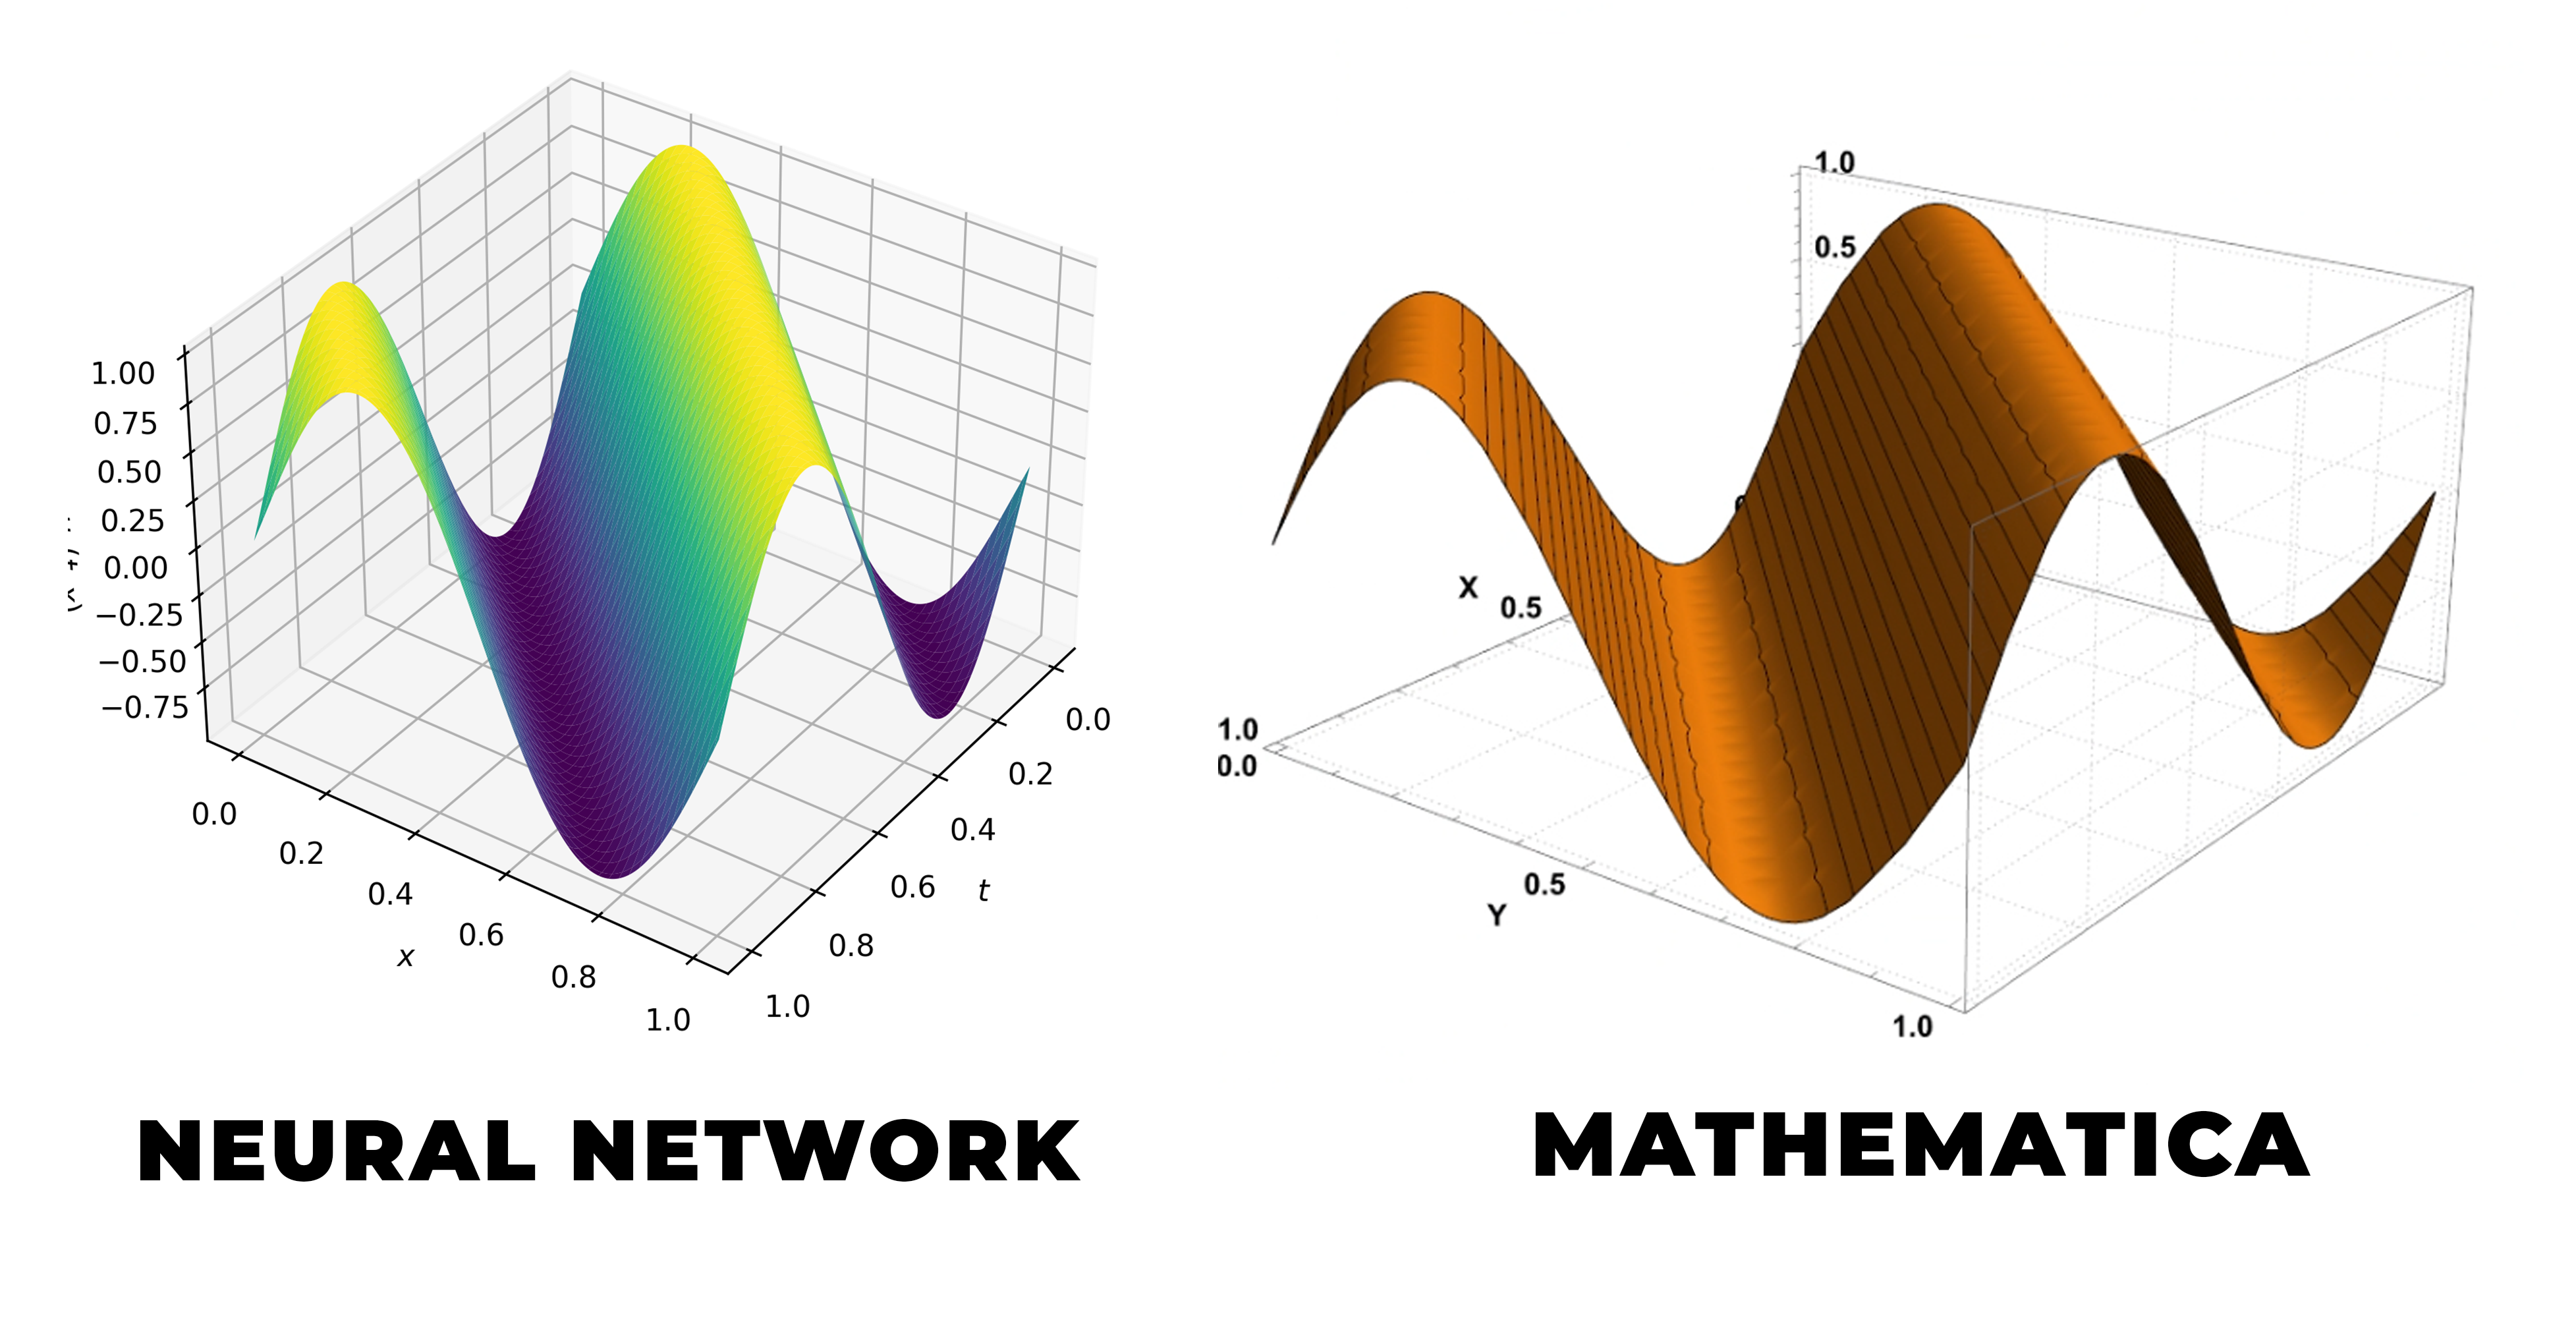
\includegraphics[width=1\linewidth]{src/Results.png}
  \end{center}

\end{frame}



%--------------------------------------------------------------
\section{Ajuste de los parámetros}
%--------------------------------------------------------------

\begin{frame}{Aprendizaje supervisado}
%-------------------------------------
\begin{itemize}
  \item En redes supervisadas, se dispone de \structure{datos de entrenamiento}, formados por un conjunto de valores de entrada $\widehat x$, junto con los resultados asociados, $\widehat y$   
  \item Es usual disponer además de \structure{datos de test}, \texttt{xtest}, \texttt{ytest}
\end{itemize}
\end{frame}

\begin{frame}{Función de coste y entrenamiento de la red neuronal}
%-------------------------------------
\begin{itemize}
  \item El proceso de \alert{entrenamiento de la red neuronal} consiste en determinar los parámetros (pesos, $w_{j,k}^{(i)}$ y desplazamientos, $b_j^{(i)}$) que minimizan un funcional, "\alert{función de coste}", sobre los datos de entrenamiento:
  $$
  \Theta^* = 
  \mbox{argmin}\{ 
  J(\Theta; \widehat x, \widehat y), \quad \Theta=\left(w_{j,k}^{(i)}, b_j^{(i)}\right)\}
  $$
\item La función de coste varía con cada tipo de red neuronal. Por ejemplo, en problemas de regresión se suelen usar mínimos cuadrados ("\structure{MSE}: minimum mean square error"):
    $$
  J(\Theta; \widehat x, \widehat y) =
  \frac1{N_{data}} \sum_{i=1}^{N_{data}}
  \left(\widehat y_i - f_{NN}(\widehat x_i)\right)^2
  $$
\end{itemize}
\end{frame}

\begin{frame}{Algoritmos de minimización}

  \begin{itemize}
    \item Dificultades para la minimización: complejidad del funcional de coste, grandes valores de $N_{data}$
    \item Enormes requerimientos de cálculo para el entrenamiento, uso de grandes ordenadores, GPUs
    \item Se suelen utilizar algoritmos de tipo \alert{descenso de gradiente}\footnote{\url{https://en.wikipedia.org/wiki/Gradient_descent}}
    \[
      \Theta_{k+1} =  \Theta_k - \lr \nabla_\Theta{J(\Theta_k;\widehat x, \widehat y)}, \quad \mbox{\lr: "Learning Rate"}
    \]
  \item Necesidad de derivar de forma eficiente: \alert{diferenciación automática}\footnote{\url{https://en.wikipedia.org/wiki/Automatic_differentiation}}
    \item Algoritmos de \alert{gradiente estocástico}\footnote{\url{https://en.wikipedia.org/wiki/Stochastic_gradient_descent}}: en cada paso, se calcula el gradiente pero sólo en un subconjunto aleatorio de datos
  \end{itemize}
\end{frame}

\end{document}


%%% Local Variables:
%%% coding: utf-8
%%% TeX-master: t
%%% mode: latex
%%% ispell-local-dictionary: "english"
%%% End:
